% Format teze zasnovan je na paketu memoir
% http://tug.ctan.org/macros/latex/contrib/memoir/memman.pdf ili
% http://texdoc.net/texmf-dist/doc/latex/memoir/memman.pdf
% 
% Prilikom zadavanja klase memoir, navedenim opcijama se podešava 
% veličina slova (12pt) i jednostrano štampanje (oneside).
% Ove parametre možete menjati samo ako pravite nezvanične verzije
% mastera za privatnu upotrebu (na primer, u b5 varijanti ima smisla 
% smanjiti 
\documentclass[12pt,oneside]{memoir}

% Compatibility fix for memoir versions affected by the
% \enlargethispage bug.
\makeatletter
\@ifundefined{@makespecialcolbox}{%
    \let\@makespecialcolbox\@make@specialcolbox
}{}
\makeatother

\usepackage{subcaption}
\usepackage{graphicx}
\graphicspath{
    {figures/auxiliary-results/}
    {figures/reviewed-tools/}
    {figures/system-design-diagrams/export/}
    {figures/system-results/}
    {figures/system-results/schematic-diagrams/export}
}

% Paket koji definiše sve specifičnosti mastera Matematičkog fakulteta
\usepackage{matfmaster}
%
% Podrazumevano pismo je ćirilica.
%   Ako koristite pdflatex, a ne xetex, sav latinički tekst na srpskom jeziku
%   treba biti okružen sa \lat{...} ili \begin{latinica}...\end{latinica}.
%
% Opicija [latinica]:
%   ako želite da pišete latiniciom, dodajte opciju "latinica" tj.
%   prethodni paket uključite pomoću: \usepackage[latinica]{matfmaster}.
%   Ako koristite pdflatex, a ne xetex, sav ćirilički tekst treba biti
%   okružen sa \cir{...} ili \begin{cirilica}...\end{cirilica}.
%
% Opcija [biblatex]:
%   ako želite da koristite reference na više jezika i umesto paketa
%   bibtex da koristite BibLaTeX/Biber, dodajte opciju "biblatex" tj.
%   prethodni paket uključite pomoću: \usepackage[biblatex]{matfmaster}
%
% Opcija [b5paper]:
%   ako želite da napravite verziju teze u manjem (b5) formatu, navedite
%   opciju "b5paper", tj. prethodni paket uključite pomoću: 
%   \usepackage[b5paper]{matfmaster}. Tada ima smisla razmisliti o promeni
%   veličine slova (izmenom opcije 12pt na 11pt u \documentclass{memoir}).
%
% Naravno, opcije je moguće kombinovati.
% Npr. \usepackage[b5paper,biblatex]{matfmaster}

% Pomoćni paket koji generiše nasumičan tekst u kojem se javljaju sva slova
% azbuke (nema potrebe koristiti ovo u pravim disertacijama)
\usepackage{pangrami}

% Paket koji obezbeđuje ispravni prikaz ćiriličkih italik slova kada
% se koristi pdflatex. Zakomentarisati ako na sistemu koji koristite ovaj
% paket nije dostupan ili ako ne radi ispravno.
\usepackage{cmsrb}

% Ostali paketi koji se koriste u dokumentu
\usepackage{listings} % listing programskog koda

\usepackage{hyperref}

\usepackage{array}
\usepackage{tabularx}

\interfootnotelinepenalty=10000

\newcolumntype{Y}{>{\raggedright\arraybackslash}X}

\setsecnumdepth{subsection}
\settocdepth{subsection}

% Datoteka sa literaturom u BibTex tj. BibLaTeX/Biber formatu
\bib{references}

% Ime kandidata na srpskom jeziku (u odabranom pismu)
\autor{Григории И. Рогов}
% Naslov teze na srpskom jeziku (u odabranom pismu)
\naslov{Развој веб алата за детекцију и анализу геномских варијација}
% Godina u kojoj je teza predana komisiji
\godina{2026}
% Ime i afilijacija mentora (u odabranom pismu)
\mentor{проф. др Јована \textsc{Ковачевић}, ванредни професор\\ Универзитет у Београду, Математички факултет}
% Ime i afilijacija prvog člana komisije (u odabranom pismu)
\komisijaA{др Мирјана \textsc{Маљковић Ружичић}, доцент\\ Универзитет у Београду, Математички факултет}
% Ime i afilijacija drugog člana komisije (u odabranom pismu)
\komisijaB{Невена \textsc{Ћирић}, асистент\\ Универзитет у Београду, Математички факултет}

% Ime i afilijacija trećeg člana komisije (opciono)
% \komisijaC{}
% Ime i afilijacija četvrtog člana komisije (opciono)
% \komisijaD{}
% Datum odbrane (obrisati ili iskomentarisati narednu liniju ako datum odbrane nije poznat)
\datumodbrane{??. септембар 2026.}

% Apstrakt na srpskom jeziku (u odabranom pismu)
\apstr{%
\pangrami
}

% Ključne reči na srpskom jeziku (u odabranom pismu)
\kljucnereci{Биоинформатика; геномска анализа; статистичка анализа секвенци; упоредна анализа секвенци; вишеструко поравнање секвенци; филогенетска анализа; генетичко растојање; систем \textit{JELICA}}

\begin{document}
% ==============================================================================
% Uvodni deo teze
\frontmatter
% ==============================================================================
% Naslovna strana
\naslovna
% Strana sa podacima o mentoru i članovima komisije
\komisija
% Strana sa posvetom (u odabranom pismu)
\posveta{posveta}
% Strana sa podacima o disertaciji na srpskom jeziku
\apstrakt
% Sadržaj teze
\tableofcontents*

% ==============================================================================
% Glavni deo teze
\mainmatter
% ==============================================================================

% ------------------------------------------------------------------------------
\chapter{Увод}
Упоредна анализа геномских секвенци има значајну улогу у истраживању генетичке разноврсности и еволуционих веза између организама. Она омогућава откривање нуклеотидних супституција, инсерција, делеција и других специфичности уочених приликом поређења нуклеотидних секвенци, као и идентификовање варијанти карактеристичних за појединачне еволуционе линије и кладе. Упркос постојању великог броја софтверских решења, многа од њих су уско специјализована, односно намењена појединачним фазама анализе или одређеним типовима организама. Узастопна примена више таквих алата у оквиру једне свеобухватне анализе повећава утрошак времена и рачунарских ресурса, а од корисника захтева и разумевање специфичности рада сваког од њих. Наведено указује на оправданост развоја интегрисаног алата за геномску анализу са интуитивним корисничким интерфејсом.

Циљ овог рада је пројектовање и развој софтверског алата \textit{JELICA} — \textit{Juxtaposing Evolutionary Lineages in Comparative Analysis} (поређење еволуционих линија у оквиру упоредне анализе), намењеног анализи више геномских секвенци. Алат обједињује проверу улазних података, поравнање секвенци, откривање геномских разлика и представљање резултата, при чему је посебна пажња посвећена поређењу еволуционих линија и клада, као и прелиминарном сврставању секвенци у одговарајуће филогенетске групе. Захтеви, кориснички сценарији и архитектонска решења алата \textit{JELICA} дефинишу се узимајући у обзир закључке добијене прегледом неколико постојећих алата за геномску анализу, након чега се у раду разматрају пројектовање, реализација и провера развијеног система.


\enlargethispage{\baselineskip}
Изворни текст рада у формату \LaTeX\ и пратећи материјали доступни су у репозиторијуму на адреси \url{https://github.com/RogovGreg/master-thesis}.

% \pangrami
% ------------------------------------------------------------------------------
\chapter{Преглед алата за геномску анализу}
У данашње време постоји велики број програмских алата намењених геномској анализи, поравнавању секвенци, откривању варијација, контроли квалитета и визуелизацији резултата. Ови алати се разликују према намени, подржаним типовима података, примењеним методама анализе, начинима представљања резултата и другим карактеристикама.

Пре развоја сопственог алата сврсисходно је размотрити неколико популарних решења и анализирати њихове основне могућности. Такав преглед омогућиће препознавање успешних приступа које би нови алат могао да користи при представљању резултата и интеракцији са корисником, а може помоћи и приликом уочавања ограничења постојећих алата и формулисања захтева за систем који се развија. Изведени закључци могу се користити при избору функционалности, структуре корисничког интерфејса и општег сценарија рада алата.


\section{Избор алата}
У овој секцији описан је поступак избора алата за даљи преглед. Најпре су дефинисани обавезни критеријуми, након чега је приказана њихова примена при формирању коначног списка алата.

\subsection{Критеријуми избора}
Као почетни извор коришћен је регистар \textit{bio.tools}, који садржи податке о програмским алатима и базама података у области биоинформатике. Сваки запис обухвата намену алата, подржане формате, тематске категорије, услове приступа, публикације и друге карактеристике. Пошто већину поменутих поља у запису попуњавају аутори алата и она нису обавезна, подаци могу бити непотпуни или застарели. Због тога је избор спроведен у две фазе: аутоматизована прелиминарна филтрација посредством \textit{API}-ја сервиса \textit{bio.tools} и накнадна ручна провера резултата.

Обавезни критеријуми избора били су:
\begin{itemize}
    \item \textbf{Доступност.} Алат мора бити јавно доступан, без потребе за коришћењем затворене инфраструктуре или добијањем посебне дозволе.
    \item \textbf{Цена.} Основна анализа мора бити бесплатна, док се бесплатна регистрација корисника сматрала прихватљивом.
    \item \textbf{Начин коришћења.} Мора бити доступан веб-интерфејс и/или званична верзија за \textit{Windows}, \textit{MacOS} или \textit{Linux}.
    \item \textbf{Формат улазних података.} Алат мора прихватати нуклеотидне секвенце у формату \textit{FASTA}.
    \item \textbf{Релевантна функционалност.} Алат мора подржавати најмање један од разматраних задатака: поравнавање секвенци, откривање варијација у односу на референтну секвенцу, поређење више секвенци или добијање основних статистичких података за дату секвенцу.
    \item \textbf{Пратећи материјали.} Морају бити доступни документација, упутство, материјали за обуку или примери улазних и излазних података.
    \item \textbf{Научне публикације.} Алат мора бити повезан са најмање једном научном публикацијом.
\end{itemize}


\subsection{Примена критеријума избора}
За прелиминарну филтрацију развијена је \textit{Python} скрипта \texttt{fetch\_biotools.py}, која је додата у репозиторијум рада. Део резултата добијених извршавањем скрипте приказан је на слици~\ref{fig:fetch_biotools_results}. Из \textit{EDAM} (енгл. \textit{EMBRACE Data and Methods} — подаци и методе пројекта \textit{EMBRACE}\footnote{\textbf{\textit{EMBRACE}} (енгл. \textit{A European Model for Bioinformatics Research and Community Education} — Европски модел за биоинформатичка истраживања и образовање заједнице) био је европски пројекат усмерен на интеграцију биоинформатичких алата, ресурса и истраживачких група.})  категорија\footnote{\textbf{\textit{EDAM} категорија} представља онтологију за стандардизовани опис и класификацију биоинформатичких ресурса према областима примене, операцијама, типовима података и форматима.} изабране су области \textit{Genomics}, \textit{Comparative genomics}, \textit{Sequence analysis}, \textit{Genetic variation}, \textit{Structural variation}, \textit{Alignment}, \textit{Gene structure} и \textit{Whole genome sequencing}. За сваку категорију су посредством \textit{API}-ја сервиса \textit{bio.tools} преузимани бесплатно доступни алати који прихватају формат \textit{FASTA} и којима је у овом сервису додељен статус \textit{Mature}\footnote{Термин \textbf{\textit{Mature}} представља вредност параметра \textit{maturity}, који означава степен развијености софтверског производа; у сервису \textit{bio.tools} разликују се вредности \textit{Emerging} (у развоју), \textit{Mature} (стабилан и добро развијен) и \textit{Legacy} (застарео или више се не одржава).}. Добијени записи су обједињени, а дупликати су уклоњени на основу идентификатора \textit{biotoolsID}.

\begin{figure}
    \centering
    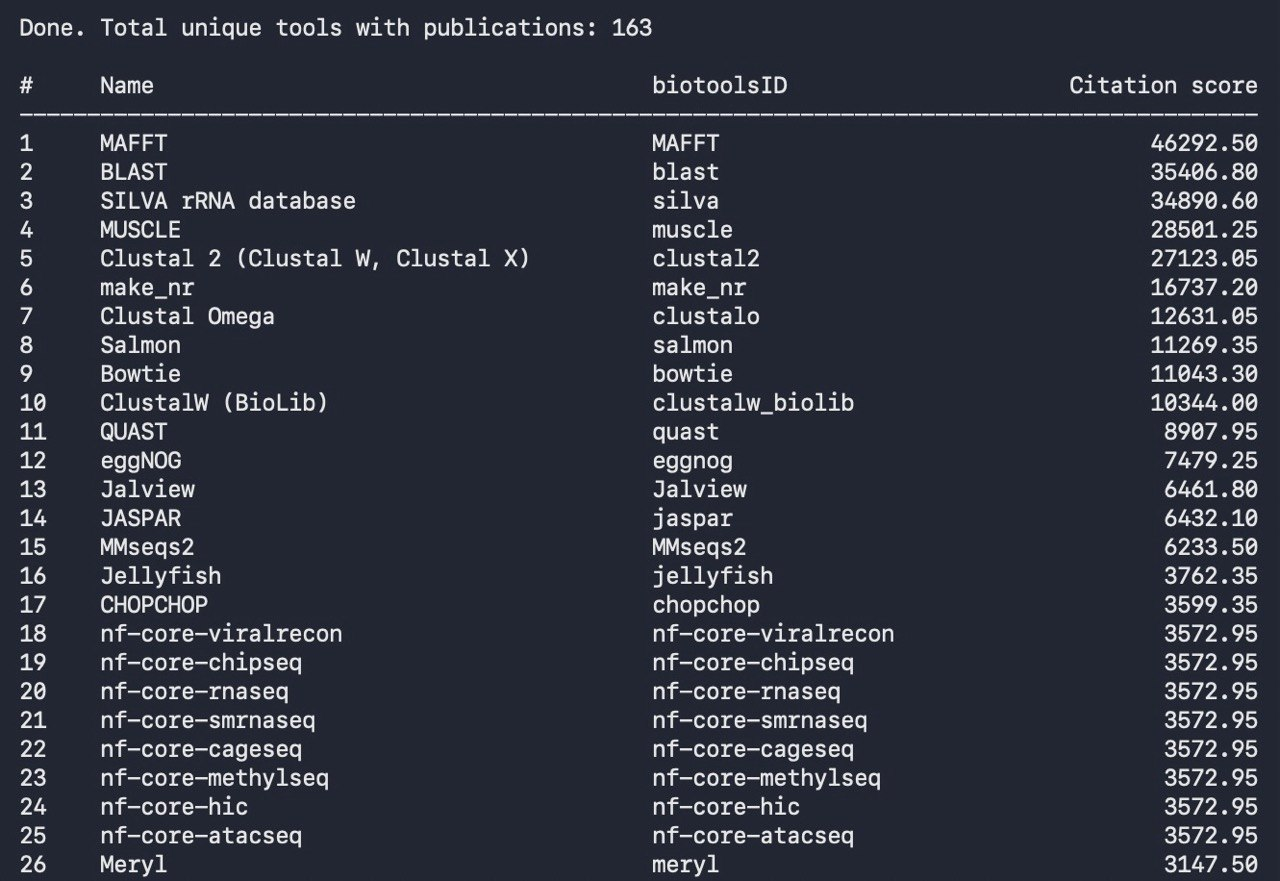
\includegraphics[width=1\linewidth]{fetch_biotools_results.jpeg}
    \caption{Резултат извршавања скрипте \texttt{fetch\_biotools.py}: првих 26 од 163 алата добијених прелиминарном филтрацијом података из регистра \textit{bio.tools} и рангираних према израчунатој оцени цитираности.}
    \label{fig:fetch_biotools_results}
\end{figure}

За рангирање алата израчунавана је оцена цитираности њихових публикација на основу података сервиса \textit{OpenAlex}\footnote{\textit{\textbf{OpenAlex}} је отворени библиографски индекс и граф научног знања који садржи податке о научним публикацијама, ауторима, институцијама, изворима и њиховим међусобним везама, доступне и посредством програмског интерфејса (\textit{API}).}. У обзир су узимани цитати из периода 2017–2026. године: за текућу годину примењиван је коефицијент \textit{1}, док се за сваку претходну годину смањивао за \textit{0,05}, до вредности \textit{0,55} за 2017. годину. Оцене свих публикација једног алата су сабиране. Алати без наведених публикација били су искључени, док је у случају немогућности преузимања података о публикацији њен допринос оцени износио нула. Након тога је списак сортиран према укупној оцени цитираности.

Коначни избор извршен је ручно и није био ограничен на првих шест позиција на ранг-листи. Из списка су искључене базе података, уско специјализовани алати, решења која су слабо повезана са темом рада и алати сличне намене. Међу алатима сличне намене предност је давана цитиранијим и боље документованим решењима.

На крају су изабрани \textit{BLAST}, \textit{Bowtie}, \textit{MAFFT}, \textit{QUAST}, \textit{Nextclade} и \textit{Clustal Omega}. Они обухватају различите задатке: претрагу сличности, мапирање на референтну секвенцу, вишеструко поравнавање, процену квалитета склопљеног генома и анализу вирусних секвенци. То омогућава разматрање различитих приступа функционалности, корисничком интерфејсу и представљању резултата.

\section{Методика прегледа алата}
Пошто разматрани алати служе за обраду различитих класа задатака, њихово поређење се не спроводи као директно поређење тачности или перформанси. Преглед се изводи према јединственој шеми, која омогућава да се упореде не сами алгоритми, већ подржани кориснички сценарији, типови улазних и излазних података, начини представљања резултата и ограничења значајна за касније пројектовање.

За сваки алат разматрају се његова основна намена, подржани типови улазних података, могућност рада са референтном секвенцом, подршка за анализу више узорака, постојање функција поравнања, претраге варијација или процене квалитета, као и начини визуелизације и извоза резултата. Посебна пажња посвећује се корисничком интерфејсу: постојању веб-верзије, \textit{CLI}-интерфејса, сложености подешавања параметара и једноставности тумачења резултата за корисника који није стручњак за конкретан алат.

Практична провера извршена је коришћењем јединственог тест скупа секвенци \textit{SARS-CoV-2}, описаног у поглављу~\ref{sec:testni-skup-podataka}. То омогућава употребу геномских секвенци истог организма при прегледу различитих алата, уз истовремено уважавање специфичности сваког од њих. За алате вишеструког поравнања коришћен је обједињени \textit{FASTA}-скуп, док су у \textit{Nextclade} учитаване само секвенце узорака, без посебног задавања референтне секвенце, јер је она унапред дефинисана изабраним скупом података самог алата. За алате усмерене на друге типове задатака, на пример \textit{Bowtie} и \textit{QUAST}, провера и опис изведени су у складу са њиховом основном наменом. На основу прегледа, за сваки алат формулишу се предности, ограничења и закључци значајни за пројектовање сопственог решења.

\section{Тестни скуп података}
\label{sec:testni-skup-podataka}
За практичну проверу разматраних алата припремљен је јединствен скуп нуклеотидних секвенци \textit{SARS-CoV-2} у формату \textit{FASTA}. Састав тестног скупа података приказан је у табели~\ref{tab:testni-skup-podataka}. Као референтна секвенца коришћен је запис \textit{NC\_045512.2}, који одговара изолату \textit{Wuhan-Hu-1}. Избор \textit{SARS-CoV-2} заснован је на релативно малој величини генома, широкој заступљености података у отвореним базама и подршци овом организму у више специјализованих алата, укључујући Nextclade. Употреба јединственог скупа података омогућава да се пореде не саме секвенце, већ карактеристике рада алата: учитавање улазних датотека, приказ резултата, подршка за поравнавање, откривање разлика, контролу квалитета и извоз података.

У скуп је укључено шест додатних записа из базе \textit{NCBI GenBank}. Они су изабрани тако да обухвате како секвенце блиске референтној, тако и касније варијанте. Узорак \textit{Sample 5 (OZ074724.1)} остављен је у скупу као пример нижег квалитета, са уочљивим бројем непознатих симбола. То омогућава процену тога колико јасно алати указују на проблеме у улазним подацима.

Уз рад је приложена архива са изворним материјалима: посебним \textit{FASTA} датотекама за референтну секвенцу и сваки узорак, обједињеним \textit{multi-FASTA} датотекама за заједничко учитавање секвенци, као и табелом са основним карактеристикама записа, укључујући \textit{accession ID}, дужину секвенце и број непознатих симбола. Такав састав архиве обезбеђује репродуцибилност анализе и омогућава употребу истог тестног скупа при разматрању различитих класа алата.

\begin{table}[htbp]
\centering
\small
\caption{Састав тестног скупа података}
\label{tab:testni-skup-podataka}

\begin{tabularx}{\textwidth}{|p{0.22\textwidth}|p{0.18\textwidth}|Y|}
\hline
\textbf{Назив узорка} & \textbf{\textit{Accession}} & \textbf{Кратак опис} \\
\hline

\textit{Reference} &
\texttt{\textit{NC\_045512.2}} &
\textit{Wuhan-Hu-1}, референтна секвенца \textit{SARS-CoV-2} \\
\hline

\textit{Sample 1} &
\texttt{\textit{PX622476.1}} &
Кина, 2020; рани узорак близак референтној секвенци \\
\hline

\textit{Sample 2} &
\texttt{\textit{OR936774.1}} &
ЈАР, 2021; линија \textit{B.1.351}, варијанта \textit{Beta} према класификацији \textit{WHO} \\
\hline

\textit{Sample 3} &
\texttt{\textit{OR939692.1}} &
ЈАР, 2021; линија \textit{B.1.617.2}, варијанта \textit{Delta} према класификацији \textit{WHO} \\
\hline

\textit{Sample 4} &
\texttt{\textit{PQ726080.1}} &
Шпанија, 2022; цела геномска секвенца \textit{SARS-CoV-2} \\
\hline

\textit{Sample 5} &
\texttt{\textit{OZ074724.1}} &
Место и година узорковања нису наведени у \textit{FASTA} заглављу. Узорак нижег квалитета са неодређеним симболима \\
\hline

\textit{Sample 6} &
\texttt{\textit{PZ368081.1}} &
САД, 2026; каснији узорак који проширује временски опсег скупа података \\
\hline

\end{tabularx}
\end{table}

\section{Преглед изабраних алата}
\subsection{Преглед алата \textit{BLAST}}
\textit{BLAST (Basic Local Alignment Search Tool)} је један од најпознатијих алата за проналажење сличности између биолошких секвенци. Прва верзија алгоритма представљена је 1990. године \cite{altschul1990blast}. За нуклеотидне секвенце користи се варијанта \textit{BLASTN}. Основни тип анализе који \textit{BLAST} покрива јесте проналажење локалне сличности између улазне секвенце и секвенци из базе података или задате референтне секвенце. Алат такође омогућава упоредно поређење секвенци, коришћење локалних база података и подешавање формата излаза, али није намењен за потпуно вишеструко поравнавање нити за готову анализу мутација.

Као улазне податке \textit{BLAST} прихвата секвенце у \textit{FASTA} формату: једну или више упитних секвенци, као и базу података или посебну \textit{subject/reference} секвенцу. За припремљени скуп података \textit{SARS-CoV-2} природан сценарио је поређење sample секвенци са референтном секвенцом \textit{NC\_045512.2}. Резултат рада представљају локална поравнања: идентификатори пронађених поклапања, координате региона, проценат идентичности, дужина поравнања, број непоклапања, празнине, \textit{E-value} и \textit{bit score}. Пример визуелног приказа добијених поравнања у \textit{NCBI MSA Viewer}-у, са укљученим режимом обележавања разлика бојом, приказан је на слици~\ref{fig:blast-results}. Корисник може радити са \textit{BLAST}-ом преко веб-интерфејса \textit{NCBI}, који је погодан за ручну проверу, или преко локалних програма \textit{BLAST+}, који су погодни за репродуцибилну и пакетну анализу.

\begin{figure}
    \centering
    \setlength{\fboxsep}{0pt}
    \setlength{\fboxrule}{0.4pt}
    \fbox{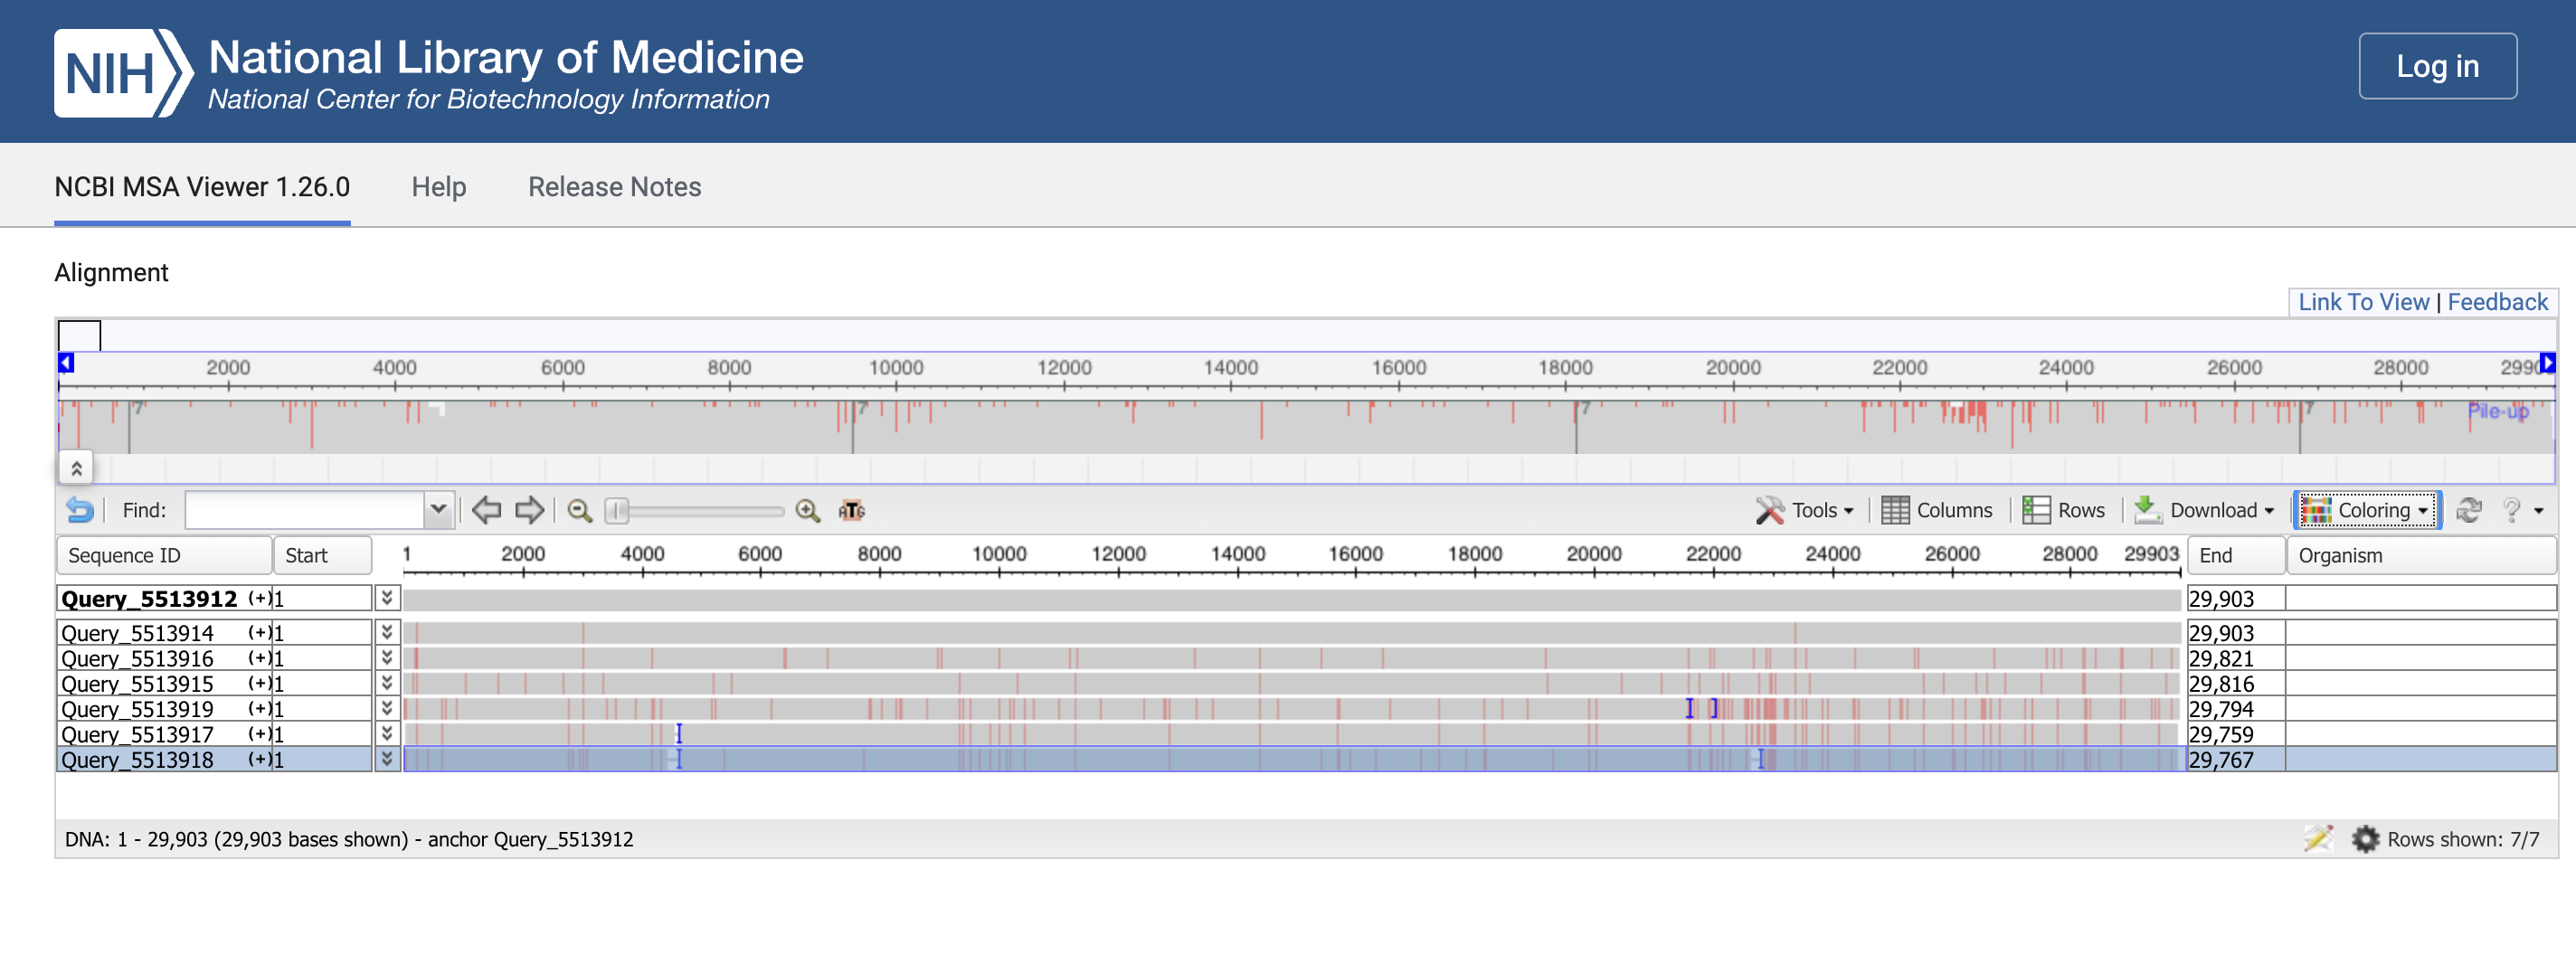
\includegraphics[width=1\linewidth]{BLAST/results.png}}
    \caption{Приказ резултата множественог поравнавања \textit{SARS-CoV-2} секвенци добијеног \textit{BLAST}-ом у \textit{NCBI MSA Viewer}-у са укљученим режимом обележавања разлика бојом у односу на референтну секвенцу.}
    \label{fig:blast-results}
\end{figure}

Јаке стране \textit{BLAST}-а су велика брзина, универзалност, широка распрострањеност, подршка за веб-интерфејс и командну линију, као и могућност да се брзо провери да ли је непозната секвенца слична очекиваном организму или референтној секвенци. Главна ограничења повезана су са тиме што \textit{BLAST} даје локална поклапања, а не готову табелу разлика у односу на референтну секвенцу. Он не формира списак \textit{SNP} и \textit{indel} промена, не агрегира промене по више узорака, не врши контролу квалитета улазних података и не повезује пронађене разлике са генима или функционалним ефектима. За пројектовани алат из овога следи да вреди преузети идеју брзог поређења са референтном секвенцом, адекватне мере сличности и могућност извоза резултата, али је потребно побољшати интерпретацију: аутоматски издвајати разлике, узимати у обзир неодређене симболе, приказивати квалитет узорака, агрегирати мутације по скупу секвенци и представљати резултате у облику погоднијем за корисника.


\subsection{Преглед алата \textit{Nextclade}}
\textit{Nextclade} је специјализовани алат за анализу већ састављених вирусних нуклеотидних секвенци. Прва стабилна верзија \textit{Nextclade} 1.0.0 објављена је 2021. године \cite{Aksamentov2021Nextclade}. Основна намена \textit{Nextclade}-а је упоређивање улазних секвенци са унапред припремљеним референтним скупом података, откривање разлика у односу на референтну секвенцу, контрола квалитета, филогенетско позиционирање и сврставање секвенци у познате филогенетске групе, односно кладе или линије. Дакле, овај алат не покрива универзалну анализу произвољних секвенци, већ специјализовани сценарио стандардизоване интерпретације вирусних секвенци.

Као улазне податке \textit{Nextclade} прихвата \textit{FASTA} датотеку са једном или више секвенци и користи изабрани референтни скуп података, који обухвата референтну секвенцу, анотацију генома са положајима гена и кодирајућих региона, филогенетско стабло и параметре анализе. Као резултат се формира табела за сваку секвенцу: списак мутација, аминокиселинске промене, делеције, инсерције, региони са недостајућим или неодређеним нуклеотидима у односу на референтну секвенцу, показатељи квалитета, упозорења, као и додељене кладе или линије. Алат омогућава извоз резултата у више формата. Корисник може радити преко веб-интерфејса, који је погодан за мање скупове података, или преко \textit{CLI} верзије, која је погоднија за обраду већих количина података и репродуцибилна покретања.

Пример резултата добијених анализом тестних \textit{SARS-CoV-2} секвенци у веб-интерфејсу \textit{Nextclade} приказан је на слици~\ref{fig:nextclade-results}.

\begin{figure}
    \centering
    \setlength{\fboxsep}{0pt}
    \setlength{\fboxrule}{0.4pt}
    \fbox{
\includegraphics[width=1\linewidth]{Nextclade/results.png}}
    \caption{Резултати анализе \textit{SARS-CoV-2} секвенци у веб-интерфејсу \textit{Nextclade}: табела са пронађеним разликама у односу на референтну секвенцу, показатељима квалитета и додељеним кладама.}
    \label{fig:nextclade-results}
\end{figure}

Снага \textit{Nextclade}-а је у томе што обједињује учитавање података, поређење са референтном секвенцом, контролу квалитета и формирање прегледног извештаја у оквиру једног корисничког сценарија. Из овог прегледа за сопствени алат корисно је преузети идеју компактне табеле резултата, аутоматске провере квалитета, јасног приказа непознатих и пропуштених позиција, извоза података и прегледног извештаја за сваки узорак. При томе не треба понављати снажну зависност од унапред припремљених скупова података: пројектовани алат треба боље да подржи рад са референтним секвенцама које задаје корисник и да раздвоји универзално поређење секвенци од специјализоване интерпретације, која је могућа само уз постојање анотација и спољних база података.

\subsection{Преглед алата MAFFT}
\textit{MAFFT} је алат за вишеструко поравнавање нуклеотидних и аминокиселинских секвенци. Прва верзија је објављена 2002. године \cite{katoh2002mafft}. У оквиру овог прегледа \textit{MAFFT} се разматра као представник класе \textit{MSA}\footnote{\textit{\textbf{MSA}} — \textit{Multiple Sequence Alignment}, вишеструко поравнавање секвенци.} алата: он не претражује секвенце у бази података и не спроводи потпуну анализу мутација, већ гради заједничко позиционо поравнавање више хомологих секвенци. Поред тога, алат подржава различите алгоритамске режиме поравнавања, локалну и веб-верзију, као и употребу у својству међукорака у сложенијим аналитичким процесима.

Као улаз \textit{MAFFT} прихвата секвенце у \textit{FASTA} формату; у веб-верзији је практичније радити са једним унапред припремљеним \textit{multi-FASTA} фајлом, што представља ограничење када за сваки узорак постоји засебан фајл. Као излаз алат даје вишеструко поравнавање, у коме су секвенце доведене на исту дужину додавањем празнина. За скуп података \textit{SARS-CoV-2} са референтном секвенцом \textit{NC\_045512.2} и више узорака такав резултат омогућава позиционо поређење секвенци и може се користити за даље откривање супституција, инсерција, делеција и непознатих региона. Ипак, \textit{MAFFT} не формира готову табелу \textit{SNP/indel} промена, не повезује промене са генима, не оцењује квалитет узорака у облику посебног извештаја и не даје биолошку интерпретацију пронађених разлика.

\begin{figure}
    \centering
    
\includegraphics[width=0.8\linewidth]{MAFFT/results.png}
    \caption{Терминалски излаз након успешног локалног извршавања \textit{MAFFT} команде за референтно поравнавање шест секвенци \textit{SARS-CoV-2} у односу на секвенцу \textit{NC\_045512.2}.}
    \label{fig:mafft-results}
\end{figure}

Снаге \textit{MAFFT}-а су подршка за стандардни \textit{FASTA} формат, добра применљивост на сличне секвенце, могућност подешавања режима поравнања (нпр. брзи режим \textit{FFT-NS-2}, прецизнији режими \textit{L-INS-i} и \textit{G-INS-i}, као и аутоматски избор режима) и могућност коришћења резултата у другим програмима. Главна ограничења нису толико повезана са квалитетом самог поравнавања, већ са корисничким сценаријем: потребно је унапред објединити засебне \textit{FASTA} фајлове, преглед дугих поравнања у веб-интерфејсу и \textit{MAFFT} \textit{MSA Viewer}-у није довољно удобан, недостаје практична навигација по позицијама разлика, као и готов извештај о променама у односу на референтну секвенцу. Из овога за пројектовани алат следи да је корисно преузети идеју стандардног улаза у \textit{FASTA} формату и позиционог поређења секвенци, али је потребно унапредити кориснички интерфејс: омогућити учитавање више засебних фајлова, аутоматско издвајање разлика у односу на референтну секвенцу, чување референтне координате, приказивање \textit{QC}\footnote{\textbf{\textit{QC}} — \textit{Quality Control}, контрола квалитета.} упозорења и представљање резултат не само као поравнавање, већ и као табеле, статистику и прегледну визуализацију.

На слици~\ref{fig:mafft-results} приказан је пример успешног локалног извршавања \textit{MAFFT} команде преко терминала у оперативном систему \textit{macOS}.


\subsection{Преглед алата \textit{Clustal Omega}}
\textit{Clustal Omega} је алат за вишеструко поравнавање секвенци, објављен 2011. године \cite{sievers2011clustalomega}. Он припада класи \textit{MSA} алата и намењен је за поређење три или више хомологних нуклеотидних или протеинских секвенци. У контексту геномске анализе, \textit{Clustal Omega} покрива задатак изградње заједничког поравнања, на основу којег се могу уочити конзервативни региони, супституције, инсерције и делеције. Додатно, алат може да прикаже једноставно стабло које приказује сличност између секвенци и матрицу сличности за сваки пар секвенци, али не врши специјализовану анотацију мутација.

Као улазне податке \textit{Clustal Omega} прихвата скуп секвенци, најчешће у \textit{FASTA} формату. Референтна секвенца може бити додата у заједнички фајл заједно са узорцима, али нема посебан статус: алат све секвенце посматра као равноправне. Као излаз корисник добија вишеструко поравнање, а у веб-верзији може да погледа и стабло и матрицу сличности. Пример резултата вишеструког поравнања у веб-интерфејсу приказан је на слици~\ref{fig:clustal-omega-results}. \textit{Clustal Omega} је доступан и преко веб-интерфејса и као \textit{CLI} апликација, што олакшава репродукцију анализе података.

\begin{figure}
    \centering
    \setlength{\fboxsep}{0pt}
    \setlength{\fboxrule}{0.4pt}
    \fbox{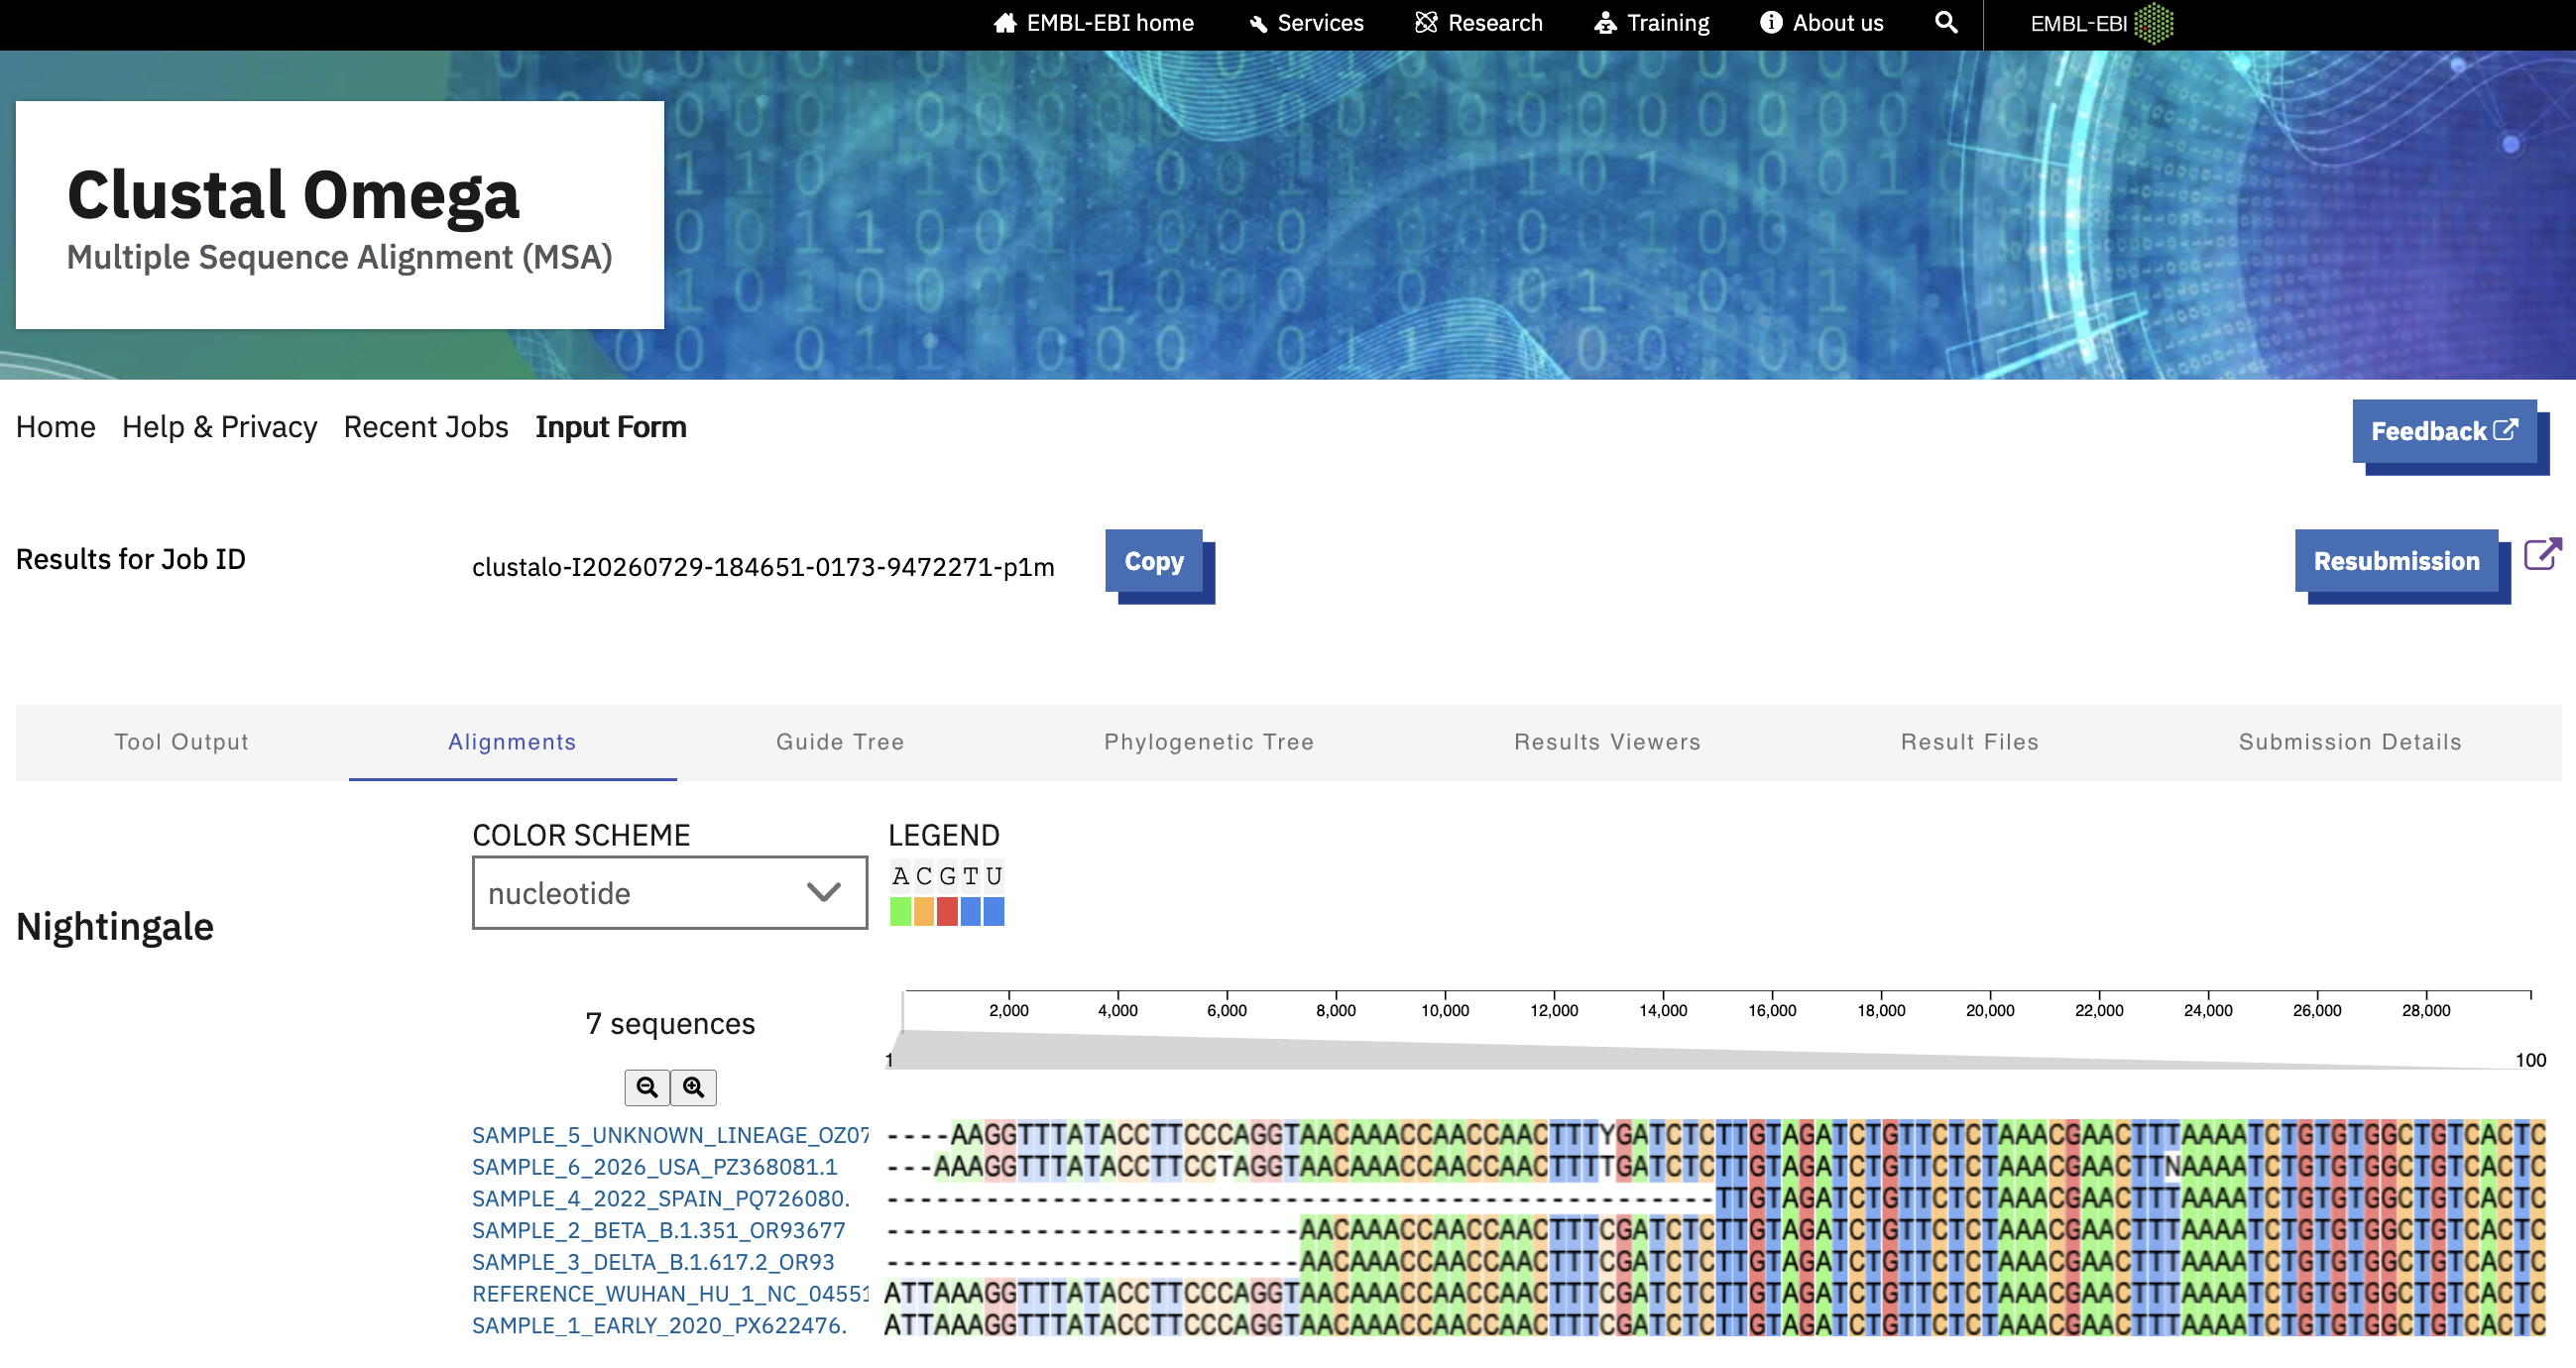
\includegraphics[width=1\linewidth]{Clustal Omega/results_alignments.png}}
    \caption{Приказ резултата множественог поравнања у веб-интерфејсу алата \textit{Clustal Omega} за референтну секвенцу \textit{SARS-CoV-2} и шест анализираних узорака}
    \label{fig:clustal-omega-results}
\end{figure}

Главне предности \textit{Clustal Omega} су једноставност употребе, подршка за стандардне формате, као и постојање веб и локалне верзије. Међутим, за задатак ове мастер тезе његов резултат представља само међукорак. \textit{Clustal Omega} не формира табелу \textit{SNP} и \textit{indel} промена у односу на изабрану референтну секвенцу, не повезује промене са генима, не оцењује квалитет узорака и не тумачи биолошко значење разлика. Из овог прегледа се за пројектовани алат може преузети идеја једноставног улаза преко \textit{FASTA} формата и прегледног приказа поравнања, али је неопходно унапредити \textit{reference-based} сценарио: јасно издвојити референтну секвенцу, аутоматски формирати извештај о разликама, узимати у обзир неодређене симболе и не ограничити се само на визуелно поравнање.


\subsection{Преглед алата \textit{Bowtie}}
\textit{Bowtie} је алат за брзо мапирање кратких секвенционих очитавања на референтни геном. Прва верзија објављена је 2009. године \cite{langmead2009bowtie}; касније је развијена проширена верзија \textit{Bowtie 2} \cite{langmead2012bowtie2}. У оквиру овог прегледа \textit{Bowtie} се разматра као представник класе алата за мапирање очитавања на референтну секвенцу (енгл. \textit{reference-based read mapping}), односно за сопостављање великог броја кратких очитавања са познатом референтном секвенцом. Његов основни сценарио је рана фаза анализе \textit{NGS} (енгл. \textit{Next-Generation Sequencing}, секвенциони подаци добијени технологијама секвенцирања нове генерације) података, после које се резултати могу користити за процену покривености, откривање варијанти, изградњу консензусне секвенце или визуализацију поравнања.

Као улазне податке \textit{Bowtie} користи референтну секвенцу, на основу које се претходно гради индекс, и скуп кратких очитавања, најчешће у формату \textit{FASTQ}\footnote{\textit{\textbf{FASTQ}} је формат за запис секвенционих очитавања који, за разлику од \textit{FASTA} формата, поред саме нуклеотидне секвенце чува и вредности квалитета за сваки прочитани симбол.}. На излазу се формира датотека са резултатима мапирања, најчешће у формату \textit{SAM} (енгл. \textit{Sequence Alignment/Map}, текстуални формат за запис резултата мапирања очитавања на референтну секвенцу), која се затим може претворити у формат \textit{BAM} (бинарна и компримована верзија формата \textit{SAM}) и користити у другим програмима. Кориснички интерфејс \textit{Bowtie} алата је командни: то није веб-апликација нити интерактивно окружење за анализу, већ нисконивоски биоинформатички алат. За припремљени скуп података \textit{SARS-CoV-2} применљивост \textit{Bowtie} алата је ограничена, јер су узорци представљени као већ састављене консензусне \textit{FASTA} секвенце, односно секвенце добијене као коначни представници анализираних узорака. Због тога је за демонстрационо покретање један узорак представљен у облику вештачки припремљених кратких очитавања, која су сопостављена са индексом изграђеним на основу референтне секвенце \textit{NC\_045512.2}. Такво покретање приказује типичан кориснички сценарио \textit{Bowtie} алата, али не представља потпуну анализу изворних секвенционих података.

\begin{figure}
    \centering
    \setlength{\fboxsep}{0pt}
    \setlength{\fboxrule}{0.4pt}
    \fbox{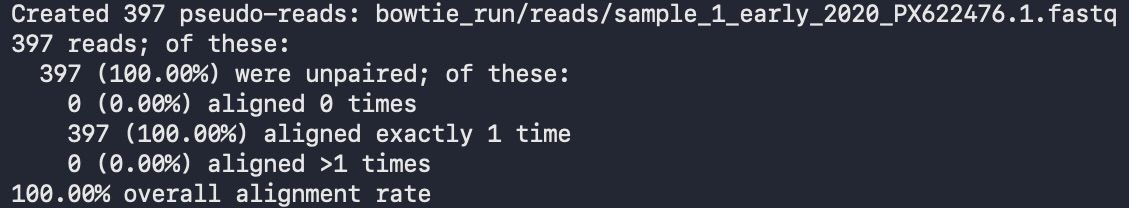
\includegraphics[width=1\linewidth]{figures/reviewed-tools/Bowtie/results.jpeg}}
    \caption{Терминалски приказ демонстрационог покретања алата \textit{Bowtie 2}: кратка вештачки припремљена очитавања једног узорка \textit{SARS-CoV-2} мапирана су на индекс изграђен на основу референтне секвенце \textit{NC\_045512.2}.}
    \label{fig:bowtie-results}
\end{figure}

Пример извршавања овог сценарија у терминалу приказан је на слици~\ref{fig:bowtie-results}. У приказаном примеру сва вештачки припремљена очитавања изабраног узорка успешно су мапирана на референтну секвенцу. Овај резултат треба тумачити као показатељ успешног мапирања очитавања, а не као доказ потпуне идентичности узорка и референце. Чак и у присуству појединачних супституција или других разлика, кратки фрагменти могу успешно да пронађу своју позицију на референтном геному. Због тога резултат \textit{Bowtie} алата сам по себи не даје кориснику готову табелу мутација, не приказује проблематичне позиције и не објашњава биолошко значење пронађених разлика.

Главне предности \textit{Bowtie} алата су велика брзина, економична употреба меморије, подршка за стандардне формате и могућност укључивања у аутоматизоване радне токове. Његова ограничења повезана су са уском специјализацијом: алат захтева посебан корак изградње индекса, оријентисан је на рад са кратким очитавањима, даје нисконивоски резултат мапирања и не формира готов кориснички извештај о разликама између састављених генома. Из овог прегледа за пројектовани алат може се преузети идеја приступа заснованог на референтној секвенци и подршка за стандардне формате, али је потребно унапредити кориснички сценарио: прихватити готове \textit{FASTA} и \textit{GenBank} секвенце, јасно издвојити референтну секвенцу, аутоматски формирати табелу \textit{SNP} и \textit{indel} промена, узимати у обзир неодређене симболе и представљати резултате не само као међуфајлове, већ и као разумљив извештај за корисника. При томе не треба понављати ограничење \textit{Bowtie} алата, при којем корисник ради добијања интерпретабилног резултата мора самостално да саставља ланац команди од више командних алата.


\subsection{Преглед алата \textit{QUAST}}
\textit{QUAST} (\textit{Quality Assessment Tool}) је алат за процену квалитета геномских асемблија, први пут објављен 2013. године у раду \textit{Gurevich et al} \cite{gurevich2013quast}. У оквиру овог прегледа он се разматра као представник класе алата за контролу квалитета геномских асемблија (\textit{genome assembly quality assessment}). Његова основна намена је процена већ добијене асемблије: њене дужине, фрагментираности, потпуности, усклађености са референтном секвенцом и могућих грешака асемблије. Додатно, алат формира графиконе, извештаје у различитим форматима и визуелизацију положаја \textit{contig}-а\footnote{\textbf{\textit{contig}} је континуирани фрагмент ДНК секвенце добијен спајањем преклапајућих секвенционих очитавања у процесу асемблије генома.} помоћу алата \textit{Icarus}.

Као улазне податке \textit{QUAST} прихвата једну или више асемблија у \textit{FASTA} формату. Референтна секвенца може бити задата додатно, али није обавезна. Без референце алат израчунава основне статистике за улазне асемблије: број \textit{contig}-а, укупну дужину, дужину највећег \textit{contig}-а, \textit{N50}\footnote{\textbf{\textit{N50}} је метрика фрагментираности асемблије: дужина таквог \textit{contig}-а да се најмање 50\% укупне дужине асемблије налази у \textit{contig}-има те дужине или дужим.}, \textit{L50}\footnote{\textbf{\textit{L50}} је број најдужих \textit{contig}-а који је потребан да би се покрило најмање 50\% укупне дужине асемблије.}, \textit{GC}-састав и број неодређених симбола. При постојању референтне секвенце додатно се израчунавају метрике поравнања: удео покривеног генома, дужина поравнатих региона, број непоклапања, инсерција и делеција, број непоравнатих \textit{contig}-а и могуће грешке асемблије. Резултати се чувају у облику директоријума са текстуалним (\texttt{.txt}), табеларним (\texttt{.csv}), \textit{HTML} и \textit{PDF} извештајима, као и додатним датотекама за визуелизацију.

За припремљени скуп података \textit{SARS-CoV-2} \textit{QUAST} је покренут у \textit{reference-based} режиму: шест секвенци у \textit{FASTA} формату предато је као посебне улазне асемблије, док је секвенца \textit{NC\_045512.2} коришћена као референтна. Пример кратког \textit{HTML} извештаја приказан је на слици~\ref{fig:quast-results}. У њему су улазне секвенце представљене као посебне асемблије, а табела садржи како метрике израчунате у односу на референцу, тако и статистике без коришћења референтне секвенце.

\begin{figure}
    \centering
    \setlength{\fboxsep}{0pt}
    \setlength{\fboxrule}{0.4pt}
    \fbox{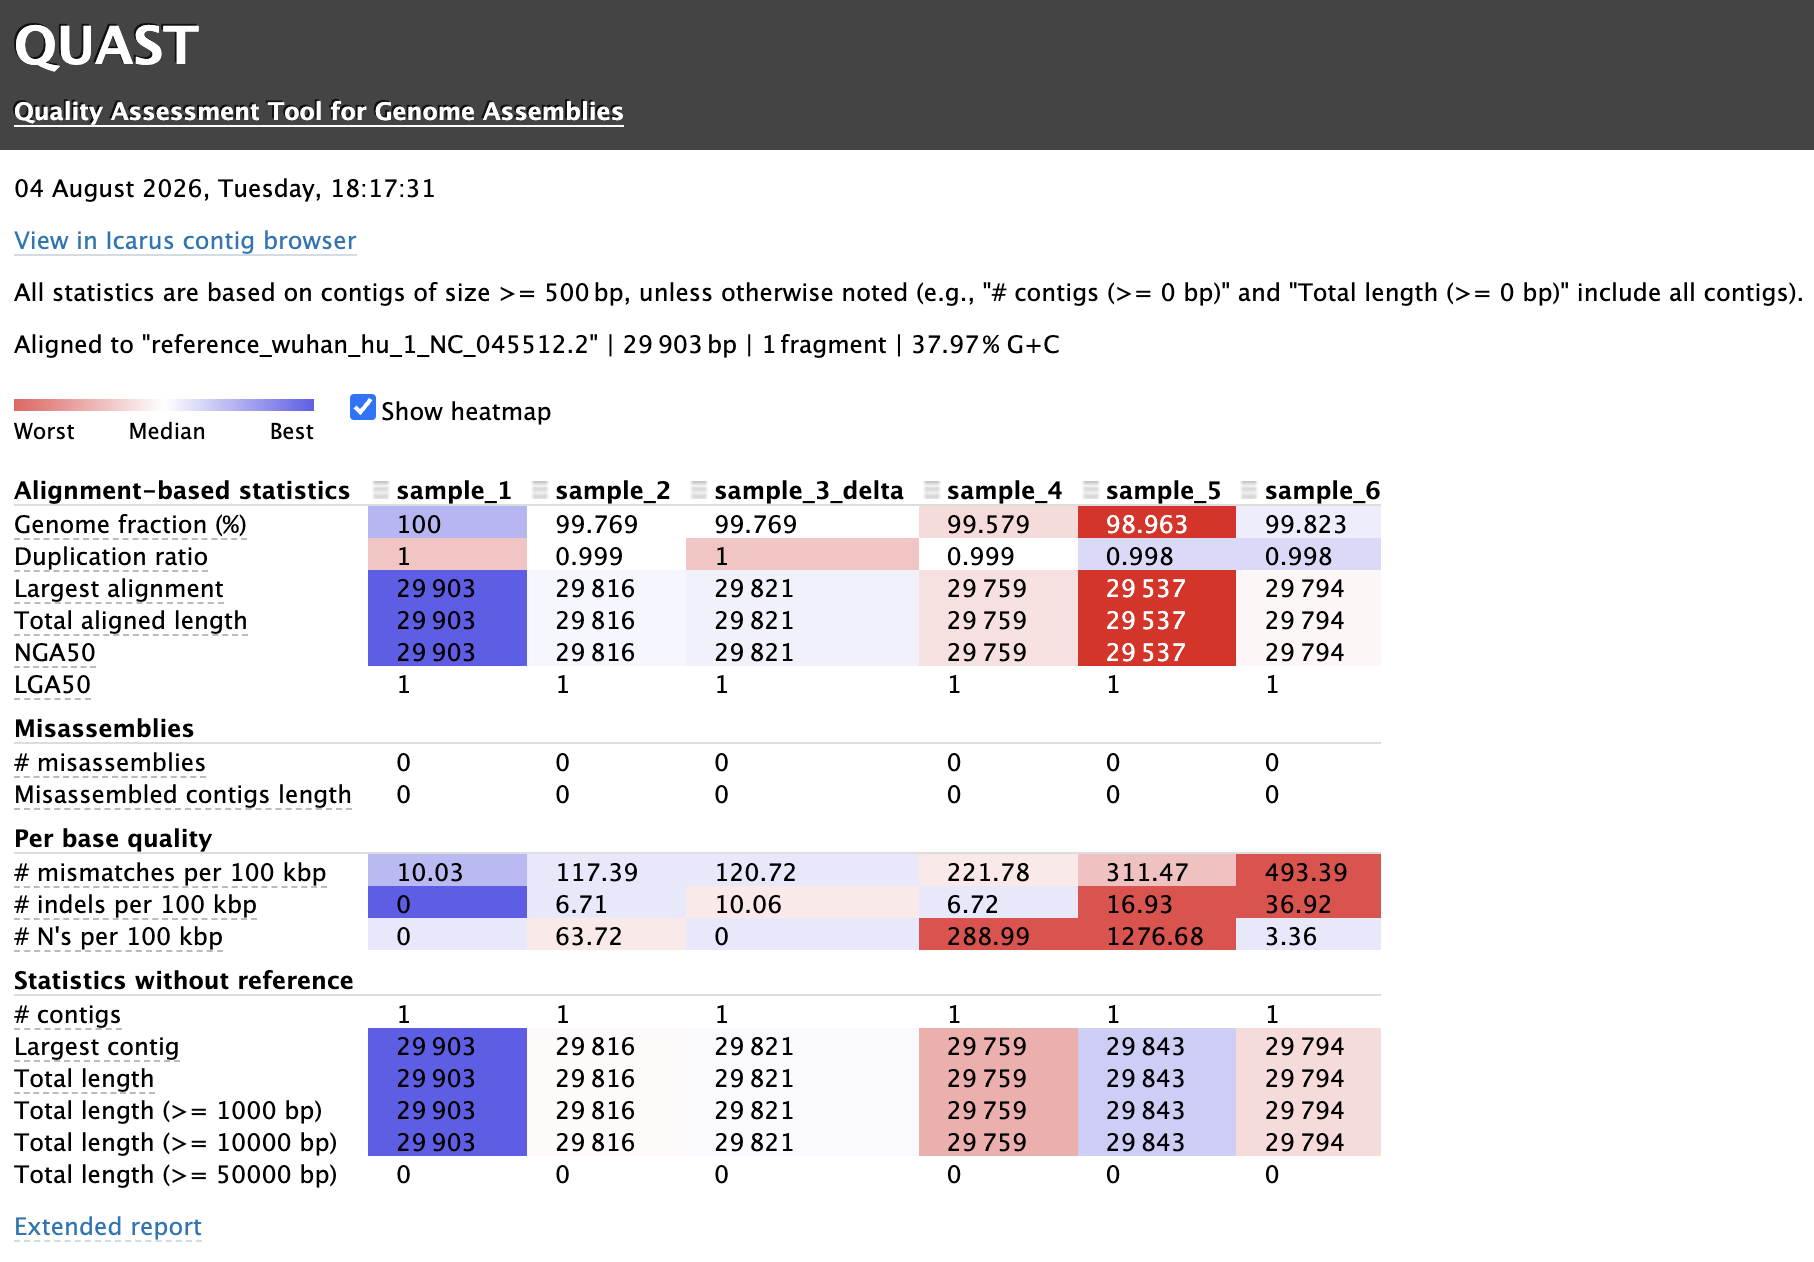
\includegraphics[width=1\linewidth]{figures/reviewed-tools/QUAST/summary_report.png}}
    \caption{Кратак \textit{HTML} извештај алата \textit{QUAST} након демонстрационог покретања на шест припремљених \textit{SARS-CoV-2} \textit{FASTA} секвенци у односу на референтну секвенцу \textit{NC\_045512.2}: приказане су упоредне метрике поравнања, контроле квалитета и основне статистике секвенци.}
    \label{fig:quast-results}
\end{figure}

Главна предност \textit{QUAST}-а је у томе што обједињује покретање анализе, израчунавање \textit{QC} метрика, формирање графикона и креирање погодног упоредног извештаја за више улазних датотека. Међутим, његова ограничења повезана су са истом том специјализацијом: алат је оријентисан на процену квалитета асемблија, а не на детаљно поређење готових нуклеотидних секвенци. \textit{QUAST} не формира потпуну табелу \textit{SNP} и \textit{indel} промена у односу на изабрану референтну секвенцу, не повезује разлике са генима, не агрегира варијанте по више узорака и не даје интерпретацију пронађених разлика. За пројектовани алат из овог прегледа вреди преузети идеју посебног \textit{QC} блока, јединствене упоредне табеле, \textit{HTML} извештаја и извоза резултата у машински читљивим форматима. При томе не треба понављати оријентацију \textit{QUAST}-а на \textit{contig-level} метрике као главни резултат: за овај рад основни објекат анализе треба да буду конкретне разлике између секвенци и референце, укључујући \textit{SNP}, \textit{indel}, пропуштене и неодређене позиције, њихове координате и збирну статистику за скуп података.


\chapter{Развој система \textit{JELICA}: пројектовање и имплементација}
\chaptermark{Развој система \textit{JELICA}}

\section{Намена и општи концепт алата}
\subsection{Намена алата}
Софтверски алат \textit{JELICA}, који се развија у оквиру овог рада, намењен је упоредној анализи секвенци целих или приближно целих генома уз узимање у обзир њихове еволуционе повезаности. Његова основна намена је обједињавање провере и припреме улазних података, статистичке и упоредне анализе, откривања геномских варијација и филогенетске анализе у јединствен аналитички ток.

Систем омогућава процену сличности и разлика између анализираних секвенци, издвајање претпостављених група генетички блиских секвенци и формирање структуираних резултата погодних за даље истраживање и обраду. Конкретни сценарији употребе алата описани су у наредном потпоглављу.

\subsection{Основни сценарији употребе}
\label{sec:basic-usage-scenarios}
Програмски алат \textit{JELICA} намењен је анализи једне или више целих геномских секвенци. Скуп операција које се извршавају зависи од броја учитаних узорака, постојања референтне секвенце и додатних података које је корисник навео. Основни сценарији употребе алата обухватају:

\begin{itemize}
    \item \textbf{Статистичку анализу појединачне геномске секвенце}, која укључује проверу њеног формата, целовитости и квалитета, одређивање дужине, нуклеотидног састава и других основних карактеристика.
    \item \textbf{Упоредну анализу више геномских секвенци}, која обухвата њихово вишеструко поравнање, откривање нуклеотидних супституција, уметања и брисања, утврђивање заједничких и јединствених варијанти, као и израчунавање показатеља сличности и разлика између узорака.
    \item \textbf{Анализу секвенци у односу на референтну секвенцу}, коју корисник задаје међу улазним секвенцама, при чему се узорци поравнавају са заједничком референтном секвенцом, а откривене разлике приказују у оквиру јединственог координатног система.
    \item \textbf{Испитивање скупа без унапред задате референтне секвенце}, при чему систем може да обрађује већ поравнате секвенце и извршава оне фазе анализе за које су испуњени неопходни предуслови. Уколико улазне секвенце нису унапред поравнате, систем у овом режиму не извршава поравнање, па се не покрећу ни фазе које захтевају поравнате секвенце.
    \item \textbf{Одређивање претпостављених еволутивних веза између узорака} на основу израчунатих генетичких растојања и конструисаног филогенетског стабла, као и аутоматско издвајање претпостављених група генетички блиских секвенци на основу матрице растојања.
    \item \textbf{Анализу група узорака које је задао корисник}, као што су линије, сојеви, географске или временске групе, уз утврђивање варијанти карактеристичних за њих и процену усклађености такве поделе са резултатима геномске анализе.
    \item \textbf{Проверу квалитета и биолошке упоредивости улазних података}, која омогућава откривање оштећених и нецелих секвенци, узорака који се значајно разликују од осталих.
    \item \textbf{Преглед и испитивање резултата анализе}, укључујући статистичке карактеристике секвенци, резултате поравнања, појединачне позиције, откривене геномске варијанте, анализиране узорке и формиране групе.
    \item \textbf{Извоз резултата} у форматима погодним за даљу обраду, визуелизацију и употребу у истраживачком раду.
\end{itemize}


\subsection{Границе функционалности и ограничења}
\textit{JELICA} ради са припремљеним геномским секвенцама које представљају целе или приближно целе геноме. Обрада сирових очитавања секвенцирања, \textit{de novo} састављање генома\footnote{Састављање генома без употребе референтне секвенце.}, аутоматска анотација непознатих генома и исправљање грешака у примарним подацима не улазе у функционалне границе тренутне верзије алата.

Резултати анализе коју \textit{JELICA} производи имају истраживачки карактер. Откривене разлике не тумаче се аутоматски као функционално значајне, патогене или раније непознате мутације. Групе које систем издвоји представљају претпостављене линије или кладе у оквиру анализираног скупа и не морају одговарати званичним класификацијама.

Поузданост резултата одређена је квалитетом, потпуношћу и упоредивошћу улазних података. Аутоматска валидација омогућава смањење ризика од некоректне анализе, али не може у потпуности заменити стручну процену. Строга ограничења обима података који се обрађују нису постављена, али стварне перформансе система зависе од доступних рачунарских ресурса, због чега повећање броја и величине секвенци може значајно продужити трајање анализе.


\section{Спецификација система \textit{JELICA}}
Спецификација система \textit{JELICA} представљена је кроз три међусобно повезане групе. \textbf{Функционална спецификација} описује предвиђене могућности система, \textbf{спецификација критеријума квалитета} одређује карактеристике квалитета и услове рада, док \textbf{спецификација формата улазних и излазних података} утврђује правила представљања, обраде и формирања података.


\subsection{Функционална спецификација}
\label{sec:functional-specification}
Функционална спецификација одређује операције које програмски алат JELICA треба да подржава и разрађује функционалности неопходне за реализацију основних сценарија употребе описаних у потпоглављу~\ref{sec:basic-usage-scenarios}. Предвиђене функције обухватају учитавање и валидацију геномских података, спровођење статистичке и упоредне анализе, филогенетску анализу, визуелизацију и извоз добијених резултата. Скуп доступних операција зависи од броја учитаних секвенци, резултата провере њиховог квалитета и упоредивости, као и од верзије апликације која се користи.


\subsubsection{Начини коришћења система}
Систем треба да буде доступан у локалној и веб-верзији. Локална верзија треба да се извршава коришћењем рачунарских ресурса корисника и да подразумевано пружа интерфејс командне линије за управљање учитавањем података, покретањем анализе и чувањем резултата. Корисник такође треба да има могућност да засебно инсталира графички интерфејс који користи функционалности локалног аналитичког језгра. Веб-верзија треба да представља апликацију у облаку, у којој се чување пројеката и извршавање аналитичких операција обављају на серверској инфраструктури система.

Основне функције система \textit{JELICA} приказане су на слици~\ref{fig:use-cases-diagram}.

\begin{figure}
    \centering
    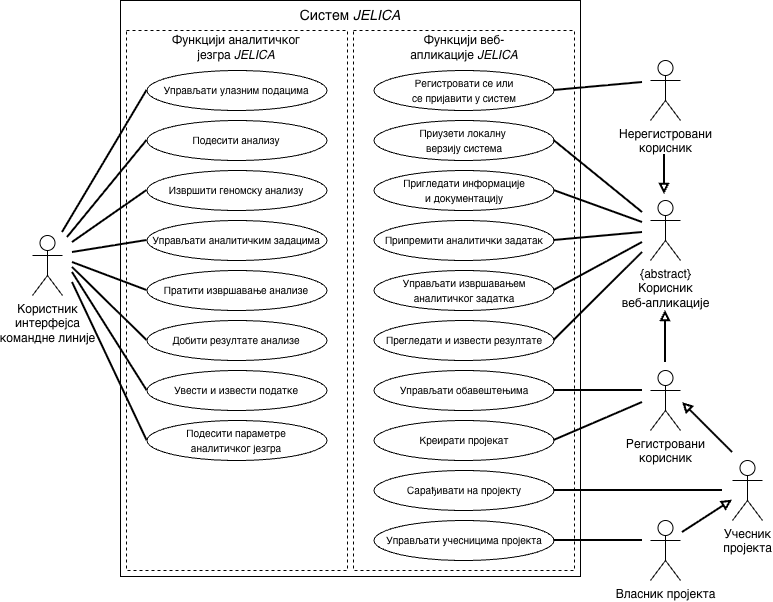
\includegraphics[width=1\linewidth]{use-cases-diagram.png}
    \caption{\textit{UML} дијаграм случајева коришћења који приказује основне функције система \textit{JELICA}.}
    \label{fig:use-cases-diagram}
\end{figure}


\subsubsection{Учитавање и валидација података}
Систем треба да омогући учитавање улазних података у форматима дефинисаним у потпоглављу~\ref{sec:specification-of-input-and-output-data-formats}. Након учитавања, систем треба да издвоји основне информације о сваком узорку, прикаже списак додатих секвенци и омогући кориснику да пре покретања анализе провери састав скупа података. Корисник треба да има могућност да уклони грешком учитан узорак, преименује га, дода или исправи метаподатке и, по потреби, одреди секвенцу која ће се користити као референтна.

Валидација сваке датотеке треба да буде започета аутоматски након њеног учитавања и да се извршава у позадини. Током њеног извршавања корисник треба да има могућност да настави са учитавањем других датотека и да ради са већ провереним узорцима. За сваку датотеку систем треба да прикаже тренутно стање обраде, резултат провере и откривене проблеме. Грешка приликом обраде једне датотеке не треба да онемогући учитавање и валидацију осталих датотека у скупу.

Пре извршавања основне анализе систем треба да спроведе вишеслојну валидацију улазних података. Она треба да обухвати проверу исправности структуре датотека, постојања секвенци у њима, коректности употребљених симбола, целовитости података и усклађености са утврђеним ограничењима. За сваку секвенцу треба израчунати основне показатеље, укључујући дужину, нуклеотидни састав, \textit{GC}-садржај, број и удео непознатих позиција (позиција означених симболом \textit{N}), као и број или учесталост појављивања \textit{k}-мера које је задао корисник. При учитавању више узорака систем такође треба да процени њихову упоредивост, препозна секвенце које се значајно разликују и могуће дупликате. Откривени проблеми треба да буду праћени порукама о грешкама или упозорењима.


\subsubsection{Спровођење геномске анализе}
\label{sec:conducting-genomic-analysis}
Геномска анализа у систему \textit{JELICA} извршава се у оквиру \textbf{аналитичког задатка}, који представља конфигурисано покретање анализе над улазним скупом секвенци. Обим и параметри анализе одређују се конфигурацијом аналитичког задатка, која је детаљније описана у потпоглављу~\ref{sec:analytical-task-configuration}.

Ако је учитана једна секвенца, систем треба да изврши њену статистичку анализу и формира преглед основних карактеристика. Функције за које је неопходно постојање више узорака у том случају не треба да буду покренуте.

Ако постоји више упоредивих секвенци и конфигурацијом је предвиђено формирање поравнања у односу на задату референтну секвенцу, систем треба да изврши њихово вишеструко поравнање. Систем такође треба да подржи анализу већ поравнатих секвенци. Ако поравнање није доступно нити се формира у оквиру задатка, фазе које зависе од њега не треба покретати. Корисник треба да има могућност да поравнање покрене засебно или да оно буде аутоматски извршено у оквиру потпуне упоредне анализе. Резултат поравнања треба да се користи као основа за даље откривање разлика, израчунавање мере сличности и филогенетску анализу. Систем треба да очува везу између позиција у изворним и поравнатим секвенцама, као и да приликом тумачења резултата узме у обзир празнине и неодређене нуклеотиде (нпр. позиције означене симболом \textit{N}).

На основу поравнања систем треба да детектује нуклеотидне супституције, инсерције и делеције. За сваку откривену варијанту треба одредити њен положај, тип, референтно и алтернативно стање, као и секвенце у којима је присутна. Систем треба да израчуна учесталост варијанти у анализираном скупу и да разликује заједничке, јединствене и разлике карактеристичне за поједине групе. Резултати треба да буду представљени у облику структуриране табеле која омогућава преглед, сортирање и филтрирање откривених варијанти према њиховим основним карактеристикама.

Систем треба да израчунава меру сличности и генетичка растојања између свих парова секвенци, формира матрицу растојања и одређује најсличније узорке и узорке који се највише разликују. На основу резултата поравнања или израчунатих растојања треба изградити филогенетско стабло које приказује претпостављене еволутивне односе између анализираних секвенци. Корисник треба да има могућност да прегледа структуру стабла и да кроз повезане приказе истражује појединачне узорке и издвојене групе, укључујући откривене геномске варијанте повезане са њима.

Поред тога, систем треба да подржава аутоматско издвајање претпостављених група генетички блиских секвенци. За сваку такву групу треба приказати њен састав, положај на филогенетском стаблу и карактеристичне геномске варијанте. Аутоматски издвојене групе треба означити као претпостављене линије, кладе или кластере и не треба их представљати као званично утврђене таксономске категорије. Ако корисник зада сопствену поделу узорака на групе, систем треба да омогући њено поређење са израчунатим генетичким растојањима и структуром стабла.


\subsubsection{Управљање аналитичким задацима}
Дуготрајне рачунске операције треба да се извршавају у облику засебних аналитичких задатака. Систем треба да приказује њихово тренутно стање и фазу извршавања, као и да омогући кориснику да прегледа резултате већ завршених међуфаза. Резултати парсирања датотека, валидације, поравнања и других ресурсно захтевних операција треба аутоматски да се чувају након завршетка одговарајуће фазе. У случају прекида аналитичког задатка систем треба да омогући његов наставак од последње успешно завршене фазе, без поновног учитавања података, поновног подешавања параметара и поновног извршавања већ завршених прорачуна.

У веб-верзији корисник треба да покреће анализу слањем захтева за креирање аналитичког задатка. Након слања захтева, задатак треба да буде постављен у ред чекања и покренут када се ослободе рачунарски ресурси сервера. Систем треба да приказује стање задатка, укључујући чекање у реду, извршавање, паузирање, успешно завршавање, завршавање са грешком и отказивање. За задатак који чека треба приказати његов тренутни положај у реду. Ако постоји довољно података, систем може додатно да прикаже процењено време почетка извршавања, при чему таква процена треба јасно да буде означена као приближна.

Корисник треба да има могућност да паузира, настави или откаже сопствени аналитички задатак. Након паузирања систем треба током утврђеног периода да омогући његов наставак без поновног проласка кроз општи ред чекања. Ако корисник не настави задатак у том периоду, његови међурезултати треба да буду сачувани, али задатак при каснијем наставку треба поново да буде постављен у ред. У случају прекида услед техничког квара, систем треба да покуша да аутоматски настави извршавање од последње сачуване фазе. Ако тренутни наставак није могућ, задатак треба поново поставити у ред без губитка већ добијених међурезултата.


\subsubsection{Приказ резултата и могућности веб-верзије}
Резултати аналитичког задатка, чији је састав дефинисан у потпоглављу~\ref{sec:specification-of-input-and-output-data-formats}, треба да буду представљени кроз више међусобно повезаних типова визуализација, као што су табеле, графици и дијаграми, чији састав и параметре корисник може да прилагођава. Промена типа визуализације пружа могућност кориснику да поступно истражује добијене резултате.

Веб-верзија система треба додатно да обезбеди кориснику лични радни простор за чување пројеката и резултата извршених аналитичких задатака. Корисник треба да има могућност да поново отвори раније креиране пројекте и другим корисницима омогући контролисан приступ изабраним пројектима или резултатима. Корисници треба да имају могућност да остављају коментаре и напомене у пројектима и анализама којима имају приступ, у складу са додељеним правима.

Јавни део веб-апликације треба да садржи документацију за инсталацију локалне верзије, упутство за коришћење система, опис подржаних метода и формата података, као и опште информације о пројекту и његовом развоју.


\subsubsection{Обавештења}
Систем треба да обавештава корисника о догађајима који не захтевају стално праћење тока извршавања аналитичког задатка. У локалној верзији корисник треба да добије обавештење на уређају након успешног завршетка аналитичког задатка или његовог прекида услед грешке. Поред тога, коначно стање операције треба да буде приказано у интерфејсу који се користи, а при раду преко интерфејса командне линије треба да буде исписано у терминалу.

Веб-верзија треба да подржава обавештења унутар апликације, обавештења прегледача, електронску пошту и слање порука путем подржаних апликација за размену порука, укључујући \textit{WhatsApp}, \textit{Viber} и \textit{Telegram}. Обавештења прегледача и спољна обавештења треба слати тек након што корисник одобри њихово примање и подеси изабрани комуникациони канал.

Обавештења у веб-верзији треба да обухвате не само промене стања аналитичких задатака већ и догађаје повезане са заједничким радом, укључујући позив у пројекат, доделу или измену права приступа, додавање коментара или напомене од стране другог корисника и друге радње повезане са пројектима којима корисник има приступ. Корисник треба да има могућност да засебно подеси канале и категорије обавештења, као и да искључи необавезна обавештења. Обавештења унутар апликације треба да буду сачувана у списку доступном кориснику, уз могућност њиховог прегледа и означавања као прочитаних.


\subsubsection{Увоз и извоз података}
Систем треба да омогући извоз резултата анализе. У зависности од врсте података, корисник треба да има могућност да сачува статистичке показатеље, табелу откривених варијанти, матрицу растојања, поравнате секвенце, филогенетско стабло и финални извештај. Извоз треба да садржи и податке неопходне за накнадно тумачење резултата и репродуковање спроведене анализе, у складу са спецификацијом излазних података из потпоглавља~\ref{sec:specification-of-input-and-output-data-formats}.

Систем такође треба да омогући извоз и поновни увоз података неопходних за наставак рада са резултатима спроведене анализе, у складу са структуром извозних података дефинисаном у потпоглављу~\ref{sec:specification-of-input-and-output-data-formats}. На тај начин треба омогућити поновну визуелизацију резултата и њихово даље истраживање без обавезног поновног извршавања већ завршених рачунских фаза.


\subsection{Спецификација критеријума квалитета система}
\label{sec:specification-of-system-quality-criteria}
Спецификација критеријума квалитета система одређује квалитативне карактеристике система \textit{JELICA} и услове извршавања предвиђених функција. Основни захтеви обухватају перформансе, поузданост, репродуцибилност резултата, употребљивост, безбедност, преносивост и проширивост.

Систем треба рационално да користи доступне рачунарске ресурсе, док дуготрајне операције не смеју да блокирају графички интерфејс. Локална верзија треба да узима у обзир карактеристике корисничког уређаја, а веб-верзија да распоређује аналитичке задатке у складу са доступним серверским ресурсима. Граничне величине улазних података и дозвољени број секвенци треба да буду одређени на основу резултата тестирања система.

Грешка при обради појединачне датотеке или аналитичког задатка не сме да доведе до губитка других података или нарушавања рада система у целини. Резултати завршених фаза обраде треба да се чувају како би се, након отказа или поновног покретања система, аналитички задатак могао наставити од последње успешно завршене фазе. Основне операције, упозорења и грешке треба евидентирати у дневнику рада, уз навођење времена, фазе обраде и одговарајућег аналитичког задатка.

Поновно извршавање анализе са истим улазним подацима, параметрима и верзијама коришћених алата треба да даје исте резултате. Уз резултате је потребно чувати параметре аналитичког задатка, податке о изабраној референтној секвенци и верзије коришћених алгоритама. Исправност основних израчунавања треба проверавати помоћу аутоматизованих тестова и контролних скупова података.

Графички интерфејси локалне и веб-верзије треба да имају сличну структуру, пружају информативне поруке о грешкама и приказују стање дуготрајних операција. Интерфејс командне линије треба да користи стабилан машински читљив формат, једнозначне кодове завршетка и структуриране поруке о току извршавања.

Веб-верзија треба да обезбеди заштићен пренос података, аутентификацију корисника, разграничење права приступа и изолацију аналитичких задатака. Геномски подаци не смеју се прослеђивати спољним сервисима без знања корисника. Локална верзија треба да омогући потпуно извршавање анализе на корисничком уређају.

Систем треба да има модуларну структуру која раздваја аналитичко језгро, интерфејс командне линије, графичке апликације и помоћне сервисе. Архитектура треба да омогући додавање нових формата података, аналитичких метода и начина представљања резултата без потпуне прераде система. Изворни кôд система треба да буде објављен у јавно доступном репозиторијуму под отвореном лиценцом, уз примену јединствених правила форматирања и аутоматске провере кода. Јавни програмски интерфејси, основни модули и нетривијални делови логике треба да буду праћени ажурном документацијом и детаљним коментарима.


\subsection{Спецификација формата улазних и излазних података}
\label{sec:specification-of-input-and-output-data-formats}
Систем треба да прихвата једну или више целих или готово целих геномских секвенци у подржаним форматима, укључујући \textit{FASTA}, \textit{GenBank} и једноставан текстуални формат. Улазни подаци могу бити учитани у облику локалних датотека или преузети из базе \textit{GenBank} на основу наведене везе или идентификатора записа. Сваком узорку треба доделити јединствени идентификатор, наведен у улазним подацима, задат од стране корисника или формиран на основу назива датотеке или \textit{GenBank} идентификатора. Метаподаци узорака нису обавезни; уколико су доступни, систем треба да их сачува ради приказивања и извоза.

Излазни подаци треба да обухватају резултате валидације, основне статистичке показатеље, вишеструко поравнање, табелу уочених разлика у поравнању, матрицу генетичких растојања између секвенци, филогенетско стабло и резултате груписања генетички блиских секвенци, уколико су одговарајуће фазе применљиве на анализирани скуп. Резултати треба да буду представљени у облику разумљивом кориснику, као и у структурираним машински читљивим форматима погодним за даљу обраду и извоз.

За целовито чување и пренос резултата аналитичког задатка систем треба да користи специјализовани формат \texttt{.jelica}. Датотека овог формата треба да садржи улазне податке, доступне метаподатке, конфигурацију аналитичког задатка, податке о коришћеним методама и верзијама система, као и добијене резултате неопходне за њихов накнадни преглед, даљу обраду и репродукцију аналитичког задатка без поновног извршавања већ завршених фаза.

\section{Пројектовање система}
\label{sec:system-design}

\subsection{Избор архитектуре система}
При пројектовању система \textit{JELICA}, основни захтев била је независност аналитичког језгра од корисничког интерфејса, као и могућност његовог коришћења у локалном и серверском окружењу. Алат треба да подржава локални и серверски режим рада, при чему обе варијанте употребе треба да буду засноване на истом аналитичком језгру система.

У складу с тим, изабрана је модуларна архитектура са издвојеним самосталним аналитичким језгром \textit{JELICA} Core. Спољне компоненте комуницирају са њим преко јединственог интерфејса, што омогућава употребу исте имплементације аналитичке функционалности у интерфејсу командне линије, десктоп и веб-апликацији, а уједно поједностављује проширивање система и његову интеграцију са другим алатима и корисничким скриптовима.

За организацију изворног кода изабран је монорепозиторијум, који поједностављује заједнички развој компоненти, управљање верзијама и дељење модула и компоненти између различитих делова система. Јасна подела система на модуле омогућава даље проширивање система без значајних измена његове опште структуре.


\subsection{Општа архитектура система}
\label{sec:general-system-architecture}
Општа архитектура система \textit{JELICA} обухвата аналитичко језгро (модул \textbf{\textit{Core}}), интерфејс командне линије (модул \textbf{\textit{CLI}}), десктоп апликацију (модул \textbf{\textit{Desktop Application}}) и веб-платформу (модул \textbf{\textit{Web Platform}}). \textit{Core} обједињује интерне модуле задужене за припрему података, управљање задацима, извршавање аналитичког задатка и чување резултата, док спољашње компоненте обезбеђују различите начине интеракције са системом. Општа архитектура програмског алата \textit{JELICA} и међусобни односи његових главних компоненти приказани су на \textit{UML} дијаграму компоненти~\ref{fig:component-diagram}.

\begin{figure}
    \centering
    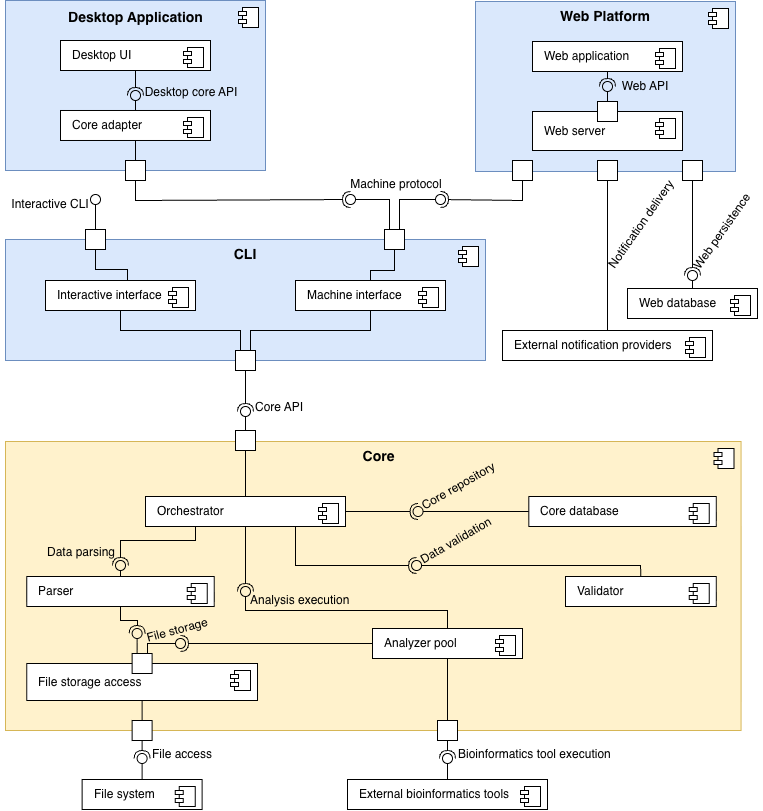
\includegraphics[width=1\linewidth]{component-diagram.png}
    \caption{Дијаграм компоненти програмског система \textit{JELICA}}
    \label{fig:component-diagram}
\end{figure}

Управљање распоређивањем аналитичких задатака у оквиру модула \textit{Core} обавља компонента \textbf{\textit{Scheduler}}. Она организује ред задатака, примењује правила приоритета и додељује задатке расположивим инстанцама радних процеса. Редоследом аналитичких фаза у оквиру конкретног покретања задатка управља оркестратор (\textit{\textbf{Orchestrator}}), који је детаљније описан у одељку о реализацији система. Модул \textit{Core} пружа јединствени програмски интерфејс преко којег спољашњи интерфејси користе функције аналитичког језгра.

Пријем и материјализацију улазних података обавља компонента \textbf{\textit{Input acquirer}}, која препознаје различите типове извора, преузима удаљене записе, обрађује локалне датотеке и директоријуме и смешта улазне податке у радни простор аналитичког задатка. Након тога компонента \textbf{\textit{Input processor}} координише парсирање, инспекцију и валидацију секвенци. Компонента \textbf{\textit{Parser}} претвара записе из подржаних формата у нормализовану интерну репрезентацију. Под \textbf{нормализованом репрезентацијом секвенце} подразумева се јединствен запис секвенце, независан од начина уноса и изворног формата, у ком су назив узорка, нуклеотидни низ, изворни идентификатори и пратећи метаподаци сведени на структуру коју могу да користе наредне компоненте система. Компонента \textbf{\textit{Sequence inspector}} у једном пролазу анализира нормализоване секвенце и прикупља њихове основне статистичке карактеристике, док компонента \textbf{\textit{Validator}} на основу резултата парсирања и инспекције проверава исправност појединачних записа и погодност целог скупа за даљу анализу. \textbf{\textit{Input processor}} такође управља дедупликацијом секвенци, одређивањем референтног узорка и формирањем међурезултата за наредне фазе обраде.

Извршавање аналитичких задатака обавља скуп радних извршилаца (компонента \textbf{\textit{Worker pool}}), којима планер додељује задатке за извршавање. Сваки радни извршилац обрађује додељени аналитички задатак проласком кроз дефинисане фазе аналитичког тока, користећи како алгоритме реализоване у оквиру система \textit{JELICA}, тако и специјализоване спољашње биоинформатичке алате. Ако су на располагању довољни рачунарски ресурси, више радних извршилаца може паралелно извршавати различите задатке, чиме се повећава укупна ефикасност система.

\textit{Core} обухвата регистар аналитичких задатака заснован на бази \textit{SQLite} и компоненту за приступ систему датотека. У бази података чувају се структурирани подаци о задацима, њиховим стањима, приоритетима, времену извршавања, грешкама и путањама до припадајућих конфигурација и резултата. Ревизије конфигурација, материјализовани улазни подаци, \textbf{манифести} фаза (описне датотеке које бележе статус извршавања фазе, настале датотеке и контролне суме), резултати поравнања, формирани резултати и други аналитички међурезултати чувају се у систему датотека.

Интеракција са аналитичким језгром остварује се преко интерфејса командне линије (\textit{\textbf{CLI}}), који представља главну приступну тачку за \textit{Core}. \textit{CLI} је пре свега намењен машинској интеракцији и обезбеђује стабилан програмски интерфејс за спољашње апликације, али подржава и непосредан рад корисника у интерактивном режиму. Десктоп апликација (\textit{\textbf{Desktop Application}}) представља графичку надоградњу над \textit{CLI}-јем. Веб-апликација (\textit{\textbf{Web Application}}) такође комуницира са аналитичким језгром преко \textit{CLI}-ја, али се та интеракција одвија на серверској страни: серверска инфраструктура претвара захтеве веб-интерфејса у команде машинског режима \textit{CLI}-ја и прослеђује добијене резултате назад клијентској апликацији. На тај начин је сва аналитичка логика концентрисана у оквиру \textit{Core} и не дуплира се у различитим варијантама испоруке система.

\subsection{Пројектовање аналитичког тока обраде}
\label{sec:analytical-workflow-design}
Аналитички ток обраде система \textit{JELICA} представља низ фаза обраде података које се извршавају под управљањем оркестратора. Његов састав се одређује на основу карактеристика улазних података и изабраних параметара анализе, чиме се омогућава аутоматско изостављање фаза које немају смисла за конкретан скуп података. Основне фазе аналитичког тока и избор одговарајућег сценарија обраде у зависности од броја валидних узорака и резултата валидације приказани су на слици~\ref{fig:activity-diagram}.

\begin{figure}
    \centering
    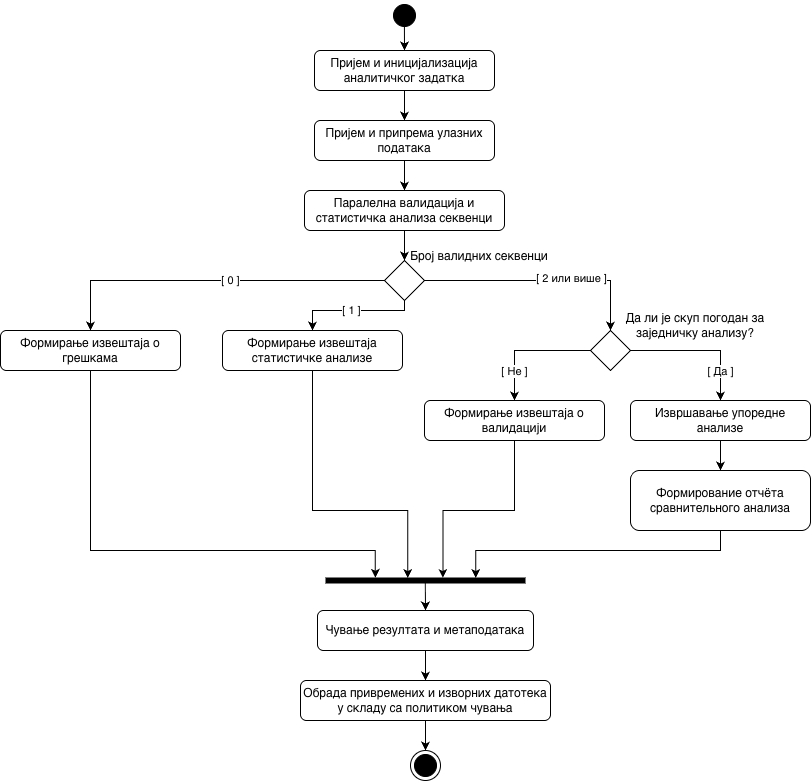
\includegraphics[width=1\linewidth]{activity-diagram.png}
    \caption{Дијаграм аналитичког тока обраде у систему \textit{JELICA}.}
    \label{fig:activity-diagram}
\end{figure}

Након пријема задатка формира се његов радни простор, а улазни извори се препознају и материјализују за даљу обраду. Припрема улазних података затим се извршава посредством компоненти описаних у потпоглављу~\ref{sec:general-system-architecture}, кроз парсирање, инспекцију и валидацију секвенци. На основу броја валидних узорака, резултата валидације и конфигурације задатка настављају се само фазе применљиве на конкретан скуп података. На пример, за један валидан узорак задржавају се резултати валидације и статистичке анализе, док се фазе упоредне анализе не покрећу.

Аналитичке задатке извршавају радни процеси компоненте \textit{Worker pool}, којима задатке додељује компонента \textit{Scheduler}, описана у потпоглављу~\ref{sec:general-system-architecture}. У оквиру конкретног покретања оркестратор управља редоследом аналитичких фаза, прати њихово стање, прослеђује информације о напретку корисничким интерфејсима и обрађује управљачке наредбе за паузирање, настављање и отказивање задатка.

Након завршетка аналитичког тока чувају се добијени резултати и припадајући метаподаци, а завршни резултати обједињују се у преносиву датотеку формата \texttt{.jelica}, чија је структура описана у потпоглављу~\ref{sec:results-model-and-format-jelica}. Привремене и изворне датотеке обрађују се у складу са изабраном политиком чувања.


\subsection{Модел података}
\label{sec:data-model}
Ради обезбеђивања уједначене размене података између компоненти система дефинисано је неколико стандардизованих модела података. Њима се описују подешавања система, параметри аналитичких задатака и структура завршног извештаја. Независно од корисничког интерфејса преко којег се креира аналитички задатак, улазни подаци и параметри преводе се у јединствену интерну репрезентацију коју користи аналитичко језгро. Начин на који се системска конфигурација и конфигурација аналитичког задатка користе при формирању потпуне конфигурације задатка, подешавању окружења аналитичког језгра и одређивању модела завршног извештаја приказан је на слици~\ref{fig:analytical-task-initialization-diagram}. Приказани поступак представља детаљнију разраду пријема и иницијализације аналитичког задатка, чије је место у целокупном аналитичком току система приказано на слици~\ref{fig:activity-diagram}.

\begin{figure}
    \centering
    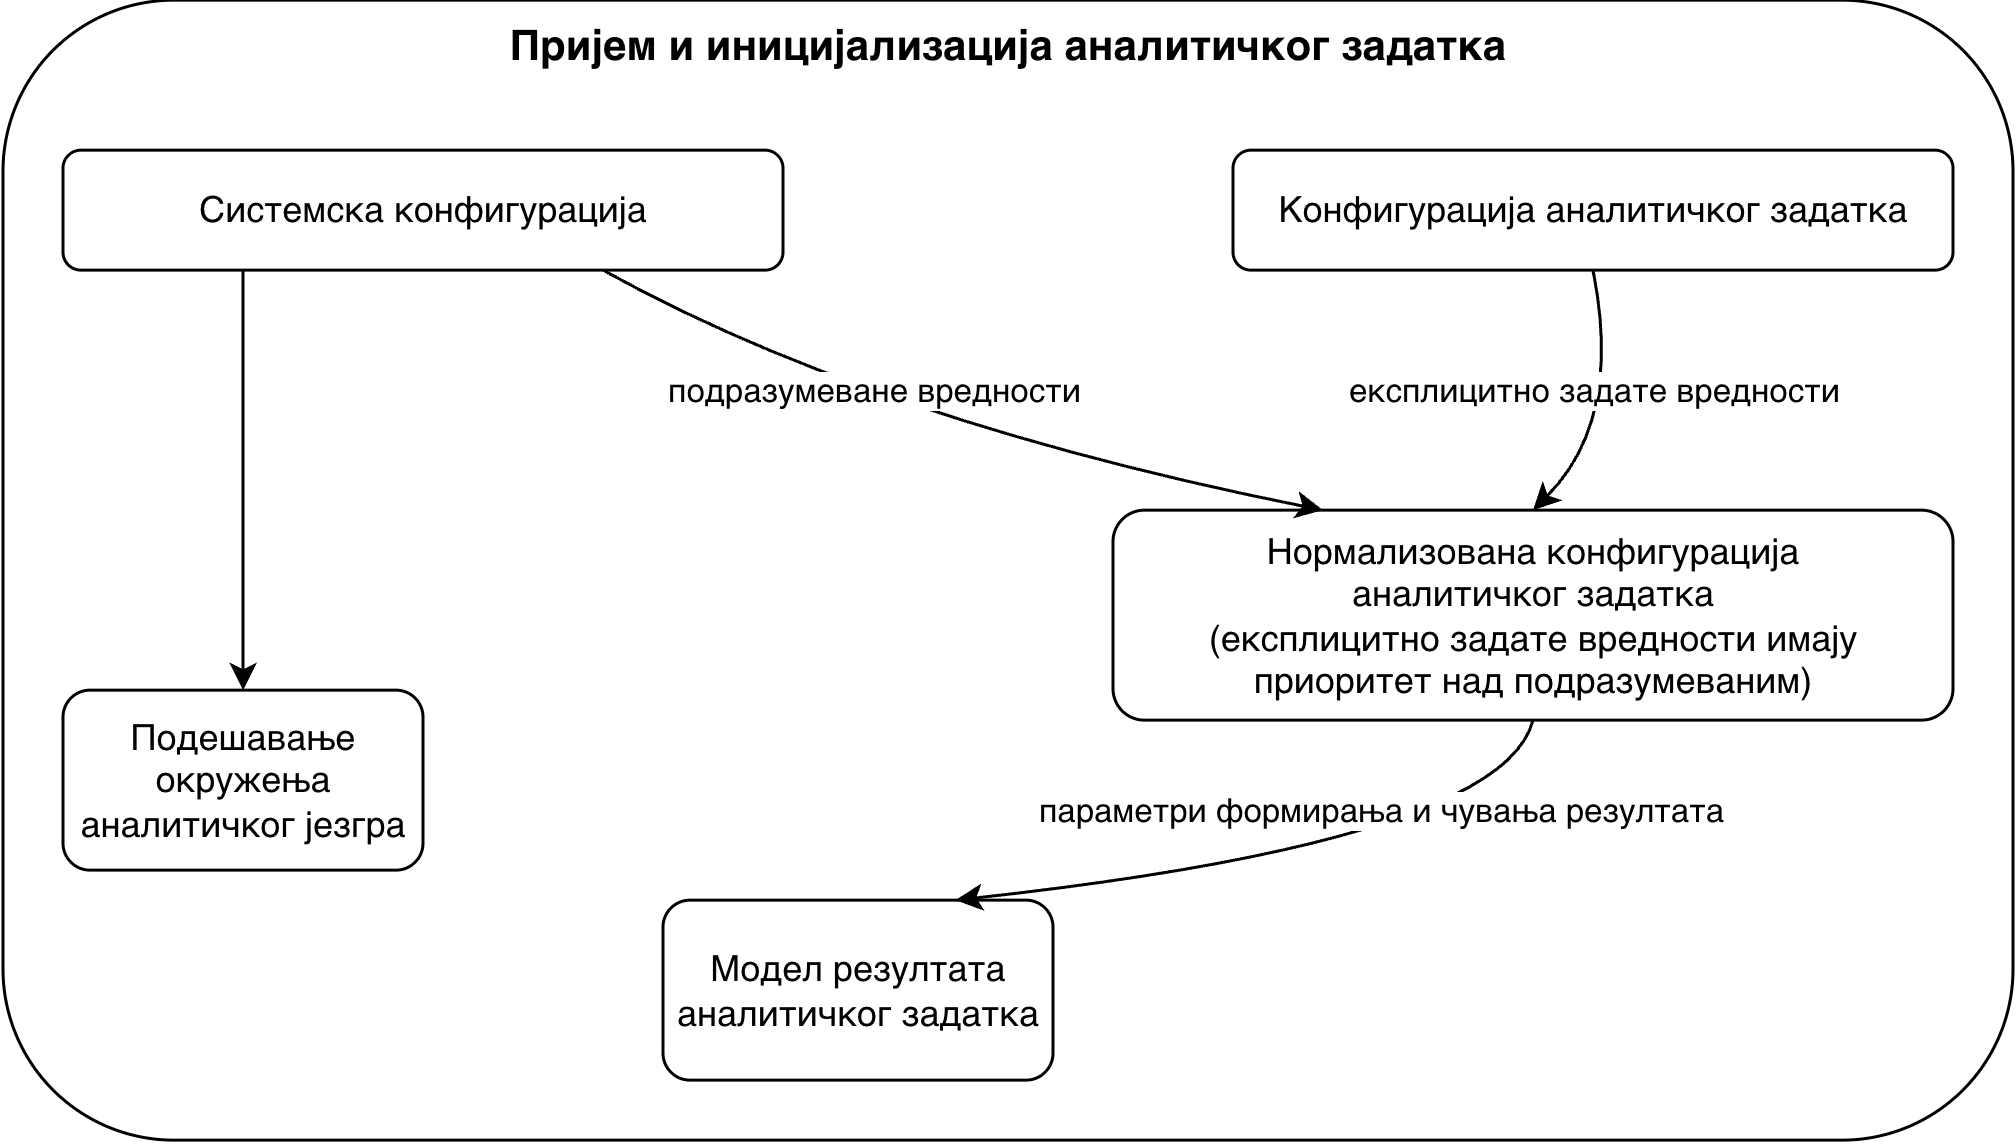
\includegraphics[width=1\linewidth]{analytical-task-initialization-diagram.png}
    \caption{Формирање потпуне конфигурације аналитичког задатка и модела завршног извештаја у оквиру пријема и иницијализације задатка.}
    \label{fig:analytical-task-initialization-diagram}
\end{figure}

\subsubsection{Конфигурација система}
Конфигурација система обухвата скуп глобалних параметара који одређују окружење у коме аналитичко језгро и остале компоненте система функционишу. За разлику од конфигурације аналитичког задатка, која описује параметре једног конкретног покретања аналитичког задатка, системска конфигурација садржи подешавања која важе за све аналитичке задатке док их корисник не измени.

У системској конфигурацији чувају се параметри који одређују локације радних директоријума, подразумеване вредности параметара који се користе при извршавању аналитичких задатака када нису експлицитно задате у конфигурацији појединачног аналитичког задатка, ограничења коришћења системских ресурса, као и друга глобална подешавања неопходна за рад система. Системска конфигурација такође садржи глобалне техничке параметре који, заједно са потпуном конфигурацијом аналитичког задатка, учествују у формирању модела завршног извештаја. Централизовано чување ових параметара омогућава њихово доследно коришћење у свим компонентама система и поједностављује администрацију и измену конфигурације.

За чување системске конфигурације изабран је формат \textit{TOML}, јер омогућава једноставно организовање глобалних параметара у прегледну хијерархијску структуру, лак је за ручно уређивање и добро је подржан у програмском језику \textit{Python}. Оваква организација поједностављује одржавање конфигурације и њено коришћење у свим компонентама система.

При покретању система проверава се постојање системске конфигурационе датотеке, која је неопходна за рад основних функционалности система. Уколико конфигурација није пронађена, систем захтева њено експлицитно навођење како би се омогућило даље извршавање. Системска конфигурација може бити иницирана и мењана путем групе команди \texttt{jelica config}, или ручно, директним уређивањем конфигурационе датотеке.

\subsubsection{Конфигурација аналитичког задатка}
\label{sec:analytical-task-configuration}
Конфигурација аналитичког задатка представља потпун опис једног аналитичког задатка и дефинише све параметре неопходне за његово извршавање. За разлику од системске конфигурације, која садржи глобална подешавања окружења за извршавање, конфигурација аналитичког задатка одређује који подаци треба да буду анализирани, које кораке аналитичког задатка је потребно извршити, са којим параметрима их треба покренути, као и на који начин треба формирати завршни извештај, укључујући његову структуру, садржај приказаних резултата и формат приказа. На тај начин, једна конфигурација у потпуности одређује ток извршавања аналитичког задатка, од учитавања улазних података до формирања завршног извештаја.

Конфигурација аналитичког задатка садржи информације о изворима улазних података, списак анализираних узорака, референтну секвенцу (уколико се користи), параметре за валидацију и претпроцесирање података, параметре за статистичку, упоредну и филогенетску анализу, као и параметре за формирање завршног извештаја. Оваква организација омогућава да се све информације неопходне за репродукцију анализе чувају у једној конфигурационој датотеци, независно од начина покретања система. Конфигурација аналитичког задатка може бити формирана ручним уређивањем конфигурационе датотеке или аутоматски, коришћењем једног од корисничких интерфејса система: интерфејса командне линије, веб-апликације или десктоп апликације.

За чување конфигурације аналитичког задатка користи се формат \textit{JSON}. Његов избор је условљен широком подршком у савременим програмским језицима, веб-технологијама и библиотекама за серијализацију података. Захваљујући томе, иста конфигурација може бити коришћена од стране интерфејса командне линије, десктоп апликације и веб-интерфејса, док аналитичко језгро увек добија јединствену интерну репрезентацију аналитичког задатка, независно од начина његовог креирања.

Коришћење јединствене конфигурације аналитичког задатка омогућава репродуковање спроведене анализе, поједностављује размену конфигурација аналитичких задатака између различитих компоненти система и омогућава поновно извршавање претходно припремљених аналитичких сценарија без потребе за поновним подешавањем параметара.

\subsubsection{Модел резултата и формат \texttt{.jelica}}
\label{sec:results-model-and-format-jelica}
Модел резултата представља структуиран машински читљив приказ стања и резултата извршавања аналитичког задатка, укључујући грешке и упозорења откривена током валидације. Овај модел не зависи од конкретног начина приказа и могу га користити аналитичко језгро, интерфејс командне линије, веб-интерфејс и десктоп апликација. На основу њега могу се формирати извештаји у форматима \textit{PDF} и \textit{HTML}, као и интерактивни прикази резултата у верзијама система са графичким корисничким интерфејсом.

За целовито чување резултата једног успешно завршеног аналитичког задатка предвиђен је специјализовани преносиви формат са екстензијом \texttt{.jelica}. Он обједињује модел резултата са улазним подацима, конфигурацијом аналитичког задатка и међурезултати аналитичких фаза неопходним за накнадни преглед и даљу обраду резултата. Посебна екстензија омогућава једнозначно препознавање датотека система \textit{JELICA}, док дефинисана структура формата омогућава њихову доследну обраду у различитим компонентама система.

Модел резултата садржи идентификатор аналитичког задатка, верзију формата резултата, податке о верзији система, опис анализираних узорака и референтне секвенце, параметре анализе примењене у конкретном аналитичком задатку, резултате провере улазних података, укључујући откривене грешке и упозорења, резултате статистичке, упоредне и филогенетске анализе, као и податке о формираним излазним датотекама. Структура и садржај модела резултата одређују се системском конфигурацијом, потпуном конфигурацијом аналитичког задатка, прослеђеним улазним подацима и корацима анализе извршеним у конкретном задатку.

Датотеке \texttt{.jelica} могу се поново учитати у систем ради провере, прегледа и формирања извештаја у траженом формату без поновног извршавања аналитичког задатка.Оваква организација раздваја чување резултата аналитичког задатка од њиховог приказа и омогућава коришћење истог модела резултата у различитим корисничким интерфејсима и форматима за извоз.


\subsection{Видови коришћења система}
\label{sec:forms-of-using-the-system}
Архитектура система \textit{JELICA} предвиђа више видова коришћења који се ослањају на заједничко аналитичко језгро \textit{JELICA Core}.

Основну варијанту представља локално коришћење преко интерфејса командне линије, намењеног пре свега аутоматизованом покретању, пакетној обради података и интеграцији у спољне радне токове. За интерактиван рад корисника обезбеђена је десктоп апликација са графичким интерфејсом, која представља надградњу над локалним компонентама система.

Поред тога, \textit{JELICA} је доступна у облику веб-верзије у облаку са клијент-сервер архитектуром. Аналитички задаци се у њој извршавају на серверској страни, док се интеракција са системом одвија преко веб-прегледача.


\section{Избор технологија и развојних алата}
Технологије за развој система \textit{JELICA} изабране су узимајући у обзир потребу за поновном употребом аналитичке логике у различитим варијантама испоруке, подршку за више оперативних система и могућност постепеног проширивања система. Додатни критеријуми били су постојање развијеног екосистема за биоинформатичка израчунавања, погодност за аутоматизацију, једноставност тестирања и могућност брзе припреме функционалне верзије алата.


\subsection{Аналитичко језгро}
Аналитичко језгро \textit{JELICA Core} реализује се на програмском језику \textit{Python}, који се широко примењује у биоинформатици и располаже великим бројем библиотека за обраду биолошких секвенци и научна израчунавања. За читање и трансформацију секвенци користи се библиотека \textit{Biopython}, док се специјализоване операције могу извршавати посредством интеграције са спољним конзолним алатима. Аналитичка логика организована је као самосталан скуп \textit{Python} модула и не зависи од корисничког интерфејса нити од начина инсталације система.


\subsection{Серверски део и \textit{API}}
Серверски део верзије у облаку развија се на програмском језику \textit{Python} уз коришћење радног оквира \textit{FastAPI}. Он пружа могућност за креирање \textit{HTTP API}-ја, проверу улазних података и аутоматско генерисање документације у формату \textit{OpenAPI}. Опис и валидација структура података обављају се помоћу \textit{Pydantic} модела.

Серверска апликација одговорна је за пријем захтева, управљање аналитичким задацима и достављање резултата, док се дуготрајне аналитичке операције извршавају у засебним радним процесима који користе \textit{JELICA Core}. Захваљујући томе, извршавање аналитичког задатка не блокира обраду осталих захтева. За чување корисника, параметара задатака, стања и метаподатака резултата користи се \textit{PostgreSQL}, док се велике улазне и излазне датотеке смештају у складиште сервера.


\subsection{Веб-интерфејс}
Веб-интерфејс реализује се на језику \textit{TypeScript} уз коришћење библиотеке \textit{React} и радног оквира \textit{Next.js}. \textit{TypeScript} омогућава статичку проверу типова и смањује вероватноћу грешака при раду са сложеним структурама резултата аналитичког задатка. \textit{React} се користи за изградњу интерактивних елемената интерфејса, док \textit{Next.js} обезбеђује организацију апликације, рутирање, изградњу и припрему верзије у облаку за инсталацију. Поред тога, избор технологија \textit{React} и \textit{TypeScript} поједностављује каснији развој десктоп апликације засноване на \textit{Electron}-у, захваљујући могућности поновне употребе значајног дела клијентског кода.

Веб-апликација комуницира са серверским делом преко \textit{HTTP API}-ја и \textit{WebSocket} веза и не садржи сопствену аналитичку логику. Њени задаци ограничени су на учитавање података, подешавање параметара, приказивање статуса извршавања у реалном времену и визуелизацију добијених резултата.


\subsection{Десктоп апликација и \textit{CLI}}
Интерфејс командне линије реализује се на програмском језику \textit{Python} уз коришћење библиотеке \textit{Typer}. Његов основни сценарио употребе представља коришћење из командне линије: покретање анализе из скрипти, аутоматизованих процеса и других програмских компоненти. Истовремено, \textit{CLI} пружа основне команде за непосредну интеракцију корисника са локалном верзијом алата.

Десктоп апликација развија се уз коришћење технологија \textit{TypeScript}, \textit{React} и \textit{Electron}. Примена \textit{Electron}-а омогућава подршку за главне десктоп оперативне системе и поновну употребу технологија и дела компоненти веб-интерфејса. Десктоп апликација представља графичку надоградњу локалног \textit{CLI}-ја и компоненте \textit{JELICA Core}, због чега се аналитички алгоритми у њој не дуплирају. За чување корисничких подешавања интерфејса и других мањих локалних података користи се уграђена база података \textit{SQLite}.


\subsection{Изградња, тестирање и испорука система}
Python зависностима и конфигурацијом пакета управља се помоћу алата \textit{uv} и датотеке \texttt{pyproject.toml}, док се зависностима TypeScript компоненти управља помоћу алата \textit{npm}.

За тестирање \textit{Python} компоненти,  како појединачно тако и интегрално, користи се \textit{pytest}. Компоненте корисничког интерфејса тестирају се помоћу алата \textit{Vitest}, док се основни кориснички сценарији веб-апликације тестирају помоћу алата \textit{Cypress}. Аутоматизоване провере, тестирање и изградња извршавају се у оквиру \textit{GitHub Actions}-а.

Серверске компоненте и неопходна инфраструктура испоручују се у \textit{Docker} контејнерима, чиме се обезбеђује репродуцибилна инсталација у окружење у облаку. Десктоп апликација пакује се у инсталационе пакете за подржане оперативне системе, док се \textit{CLI} може дистрибуирати као \textit{Python} пакет или као самосталан извршни модул.


\subsection{Развојно окружење и примена вештачке интелигенције}
Систем \textit{JELICA} развијан је у окружењу \textit{VS Code}, уз коришћење екстензија за примењене програмске језике и технологије. За управљање верзијама изворног кода користи се \textit{Git}, док је јавни репозиторијум пројекта постављен на платформи \textit{GitHub}. Ручна провера и отклањање грешака у корисничким интерфејсима спроводе се у прегледачима \textit{Chrome}, \textit{Safari}, \textit{Firefox}, \textit{Edge} и \textit{Opera}, а за проверу рада система у различитим оперативним окружењима користи се \textit{Parallels Desktop}.

Као помоћно средство при развоју користи се \textit{GitHub Copilot}, интегрисан у \textit{VS Code}, са моделима из породица \textit{Claude} и \textit{GPT-Codex}. Агенти засновани на вештачкој интелигенцији примењују се за убрзавање писања и измене програмског кода, проналажење грешака и предлагање варијанти имплементације. Сви добијени резултати накнадно се ручно проверавају, покрећу и тестирају, док је агентима онемогућен приступ \textit{Git} операцијама и самостално евидентирање измена. \textit{GitHub Copilot} се такође користи за аутоматизовани прелиминарни преглед измена на платформи \textit{GitHub}, а веб-верзија алата \textit{ChatGPT} као помоћ при пројектовању и провери архитектонских решења. Коначни избор решења и одговорност за њихову исправност остају на аутору система.


\section{Имплементација система \textit{JELICA}}
У овом потпоглављу описана је имплементација архитектонских решења представљених у потпоглављу~\ref{sec:system-design}, од организације изворног кода и управљања аналитичким задацима до реализације аналитичких фаза, чувања резултата и корисничких интерфејса.


\subsection{Организација имплементације система}
Имплементација система обухвата аналитичко језгро, интерфејс командне линије, веб-платформу и десктоп апликацију, као и заједничке моделе података, конфигурацију радног простора и аутоматизоване тестове. Компоненте написане на програмском језику \textit{Python} обједињене су у заједнички развојни радни простор, док су корисничке апликације организационо раздвојене од аналитичке имплементације. Изворни код система јавно је доступан у \textit{GitHub} репозиторијуму: \texttt{https://github.com/RogovGreg/jelica}.

Централни део имплементације представља пакет \textit{jelica-core}. Његове јавне операције користе интерфејс командне линије, серверски део веб-платформе и интеграциони слој десктоп апликације. Сваки интерфејс самостално претвара кориснички унос у одговарајући захтев и структуриране резултате језгра у облик погодан за даљу употребу у одговарајућем интерфејсу.

За размену података између компоненти користе се заједнички модели који дефинишу структуру конфигурација, аналитичких задатака и резултата.

Коректност имплементације проверава се аутоматизованим тестовима који обухватају кључне модуле система, као и њихово заједничко функционисање.


\subsection{Модел аналитичког задатка и управљање извршавањем}
У зависности од конфигурације, аналитички задаци могу да обухвате статистичку анализу једне секвенце, али и потпуну упоредну анализу скупа секвенци, као што је описано у потпоглављу~\ref{sec:conducting-genomic-analysis}.

Модел извршавања аналитичких задатака, чије су основне компоненте и њихове улоге описане у потпоглављу~\ref{sec:general-system-architecture}, имплементиран је у пакету \textit{jelica-core}. Језгро пружа јединствен скуп операција за креирање, покретање, паузирање, настављање и отказивање задатка, као и за добијање његовог тренутног стања.

Приликом креирања аналитичког задатка конфигурација описана у потпоглављу~\ref{sec:analytical-task-configuration} проверава се и обједињује са применљивим за овај задатак параметрима системске конфигурације, након чега језгро формира нормализовани приказ параметара који се стварно користе. Након успешне провере вредности параметара и формирања тог приказа, задатку се додељује јединствени идентификатор, креира се засебан радни директоријум, а нормализована конфигурација се у њему чува као датотека у формату \textit{JSON}. Уколико иницијализација задатка не може да буде завршена, подаци настали током њеног извршавања се уклањају, чиме се спречава креирање непотпуних аналитичких задатака.

Аналитички задатак представља трајни ентитет који повезује конфигурацију захтеваног задатка, његово стање према моделу из табеле~\ref{tab:analytical-task-states} и податке о извршавању. Интерни метаподаци о аналитичким задацима, као што су идентификатор задатка, тренутно стање, путања до радног директоријума и подаци о извршавању, чувају се у регистру задатака, у бази података креираној помоћу система за управљање базама података \textit{SQLite}. На тај начин омогућавају се очување стања и управљање задацима након поновног покретања система.

\begin{table}[htbp]
\centering
\caption{Стања аналитичког задатка}
\label{tab:analytical-task-states}
\begin{tabular}{|l|l|p{0.52\textwidth}|}

\hline
\textbf{Стање} & \textbf{Тип} & \textbf{Значење} \\

\hline
\texttt{waiting} & Основно & Задатак је креиран и чека покретање. \\

\hline
\texttt{queued} & Основно & Задатак је у реду и чека доступан радни процес. \\

\hline
\texttt{running} & Основно & Задатак се активно извршава. \\

\hline
\texttt{pause\_requested} & Прелазно & Примљен је захтев за контролисано паузирање. \\

\hline
\texttt{preemption\_requested} & Прелазно & Задатак треба да уступи ресурс задатку вишег приоритета. \\

\hline
\texttt{paused} & Основно & Извршавање је паузирано и може бити настављено. \\

\hline
\texttt{cancel\_requested} & Прелазно & Примљен је захтев за контролисано отказивање. \\

\hline
\texttt{completed} & Завршно & Задатак је успешно завршена. \\

\hline
\texttt{failed} & Завршно & Извршавање је завршено због грешке. \\

\hline
\texttt{cancelled} & Завршно & Извршавање је отказано пре завршетка. \\

\hline
\texttt{deletion\_requested} & Прелазно & Примљен је захтев за контролисано брисање задатка. \\

\hline
\end{tabular}
\end{table}

Креирани задаци смештају се у ред за извршавање. Планер (\textit{\textbf{Scheduler}}) бира задатке који чекају на основу њиховог приоритета, редоследа пристизања и броја расположивих радних процеса компоненте \textit{Worker pool}. Пре покретања задатка, планер у оквиру једне трансакције мења стање изабраног задатка, чиме се спречава да исти аналитички задатак буде истовремено додељен већем броју радних процеса. Када су сви расположиви радни процеси заузети, задатак остаје у реду све док се не ослободи неки од њих или док, у складу са правилима приоритета, активни задатак нижег приоритета контролисано не уступи свој радни процес.

За свако покретање или настављање аналитичког задатка формира се засебно окружење за извршавање (\textit{\textbf{Runtime}}). Ово окружење постоји само током текуће обраде и повезује податке који се трајно чувају у регистру задатака и радном директоријуму задатка са привременим подацима неопходним за извршавање. У њега спадају, на пример, учитана нормализована конфигурација, подаци о текућој фази аналитичког задатка, информације о напретку, привремени подаци који настају током појединачних фаза и ознаке команди за управљање извршавањем, којима се тражи паузирање, настављање или отказивање задатка. Приликом настављања раније паузираног задатка или поновног покретања задатка који је претходно отказан или завршен грешком формира се ново окружење за извршавање, али трајни идентификатор аналитичког задатка остаје непромењен. 

Ток извршавања аналитичког задатка координише оркестратор (\textit{\textbf{Orchestrator}}). Приликом покретања конкретног аналитичког задатка формира се објекат текућег извршавања (\textit{\textbf{Job}}), који планер додељује једном од расположивих радних процеса компоненте \textit{Worker pool} (\textit{\textbf{Worker instance}}). Додељени радни процес затим редом извршава фазе аналитичког задатка које су предвиђене његовом конфигурацијом и применљиве на улазни скуп. При настављању аналитичког задатка оркестратор проверава међурезултати и манифесте претходних фаза у радном директоријуму задатка и не понавља фазе чији су резултати већ успешно формирани и евидентирани. Однос између основних елемената који учествују у извршавању аналитичког задатка приказан је на слици~\ref{fig:task-execution-model-schematic}.

\begin{figure}
    \centering
    
\includegraphics[width=1\linewidth]{task-execution-model-schematic.png}
    \caption{Модел извршавања аналитичког задатка у систему \textit{JELICA}}
    \label{fig:task-execution-model-schematic}
\end{figure}

Команде за управљање извршавањем аналитичког задатка, као што су паузирање, настављање и отказивање, обрађују се централизовано, док се прелази између стања задатка спроводе тек након провере његовог тренутног стања. На тај начин спречавају се недозвољене операције над активним или завршеним задацима.

При паузирању, отказивању или техничком прекиду аналитичког задатка чувају се резултати свих у потпуности завршених фаза. То омогућава наставак аналитичког задатка без понављања рачунски захтевних операција које су већ успешно извршене.


\subsection{Реализација аналитичког тока}
Аналитички ток пројектован у потпоглављу~\ref{sec:analytical-workflow-design} имплементиран је као скуп међусобно повезаних фаза са дефинисаним улазним подацима, конфигурацијом и резултатима које формира свака фаза. Оркестратор на основу нормализоване конфигурације аналитичког задатка одређује које се фазе извршавају у конкретном покретању.

Прва фаза, \textit{input\_acquisition}, задужена је за преузимање улазних података. Извори могу бити локалне датотеке и директоријуми, као и записи из базе \textit{NCBI GenBank} који су задати приступним бројем или \textit{URL} адресом. Након тога фаза \textit{input\_processing} проверава формат и валидност секвенци и преводи их у нормализовану интерну репрезентацију која се користи у наставку обраде. У истој фази израчунавају се основне статистичке карактеристике секвенци, укључујући дужину секвенце, садржај неодређених нуклеотида, расподелу симбола, GC садржај и, када је задато конфигурацијом, резултате претраге \textit{k}-мера. Примери израчунатих статистичких карактеристика и резултата претраге \textit{k}-мера приказани су на слици~\ref{fig:input-processing-results}.

\begin{figure}[htbp]
    \centering

    \begin{subfigure}[t]{0.49\textwidth}
        \centering
        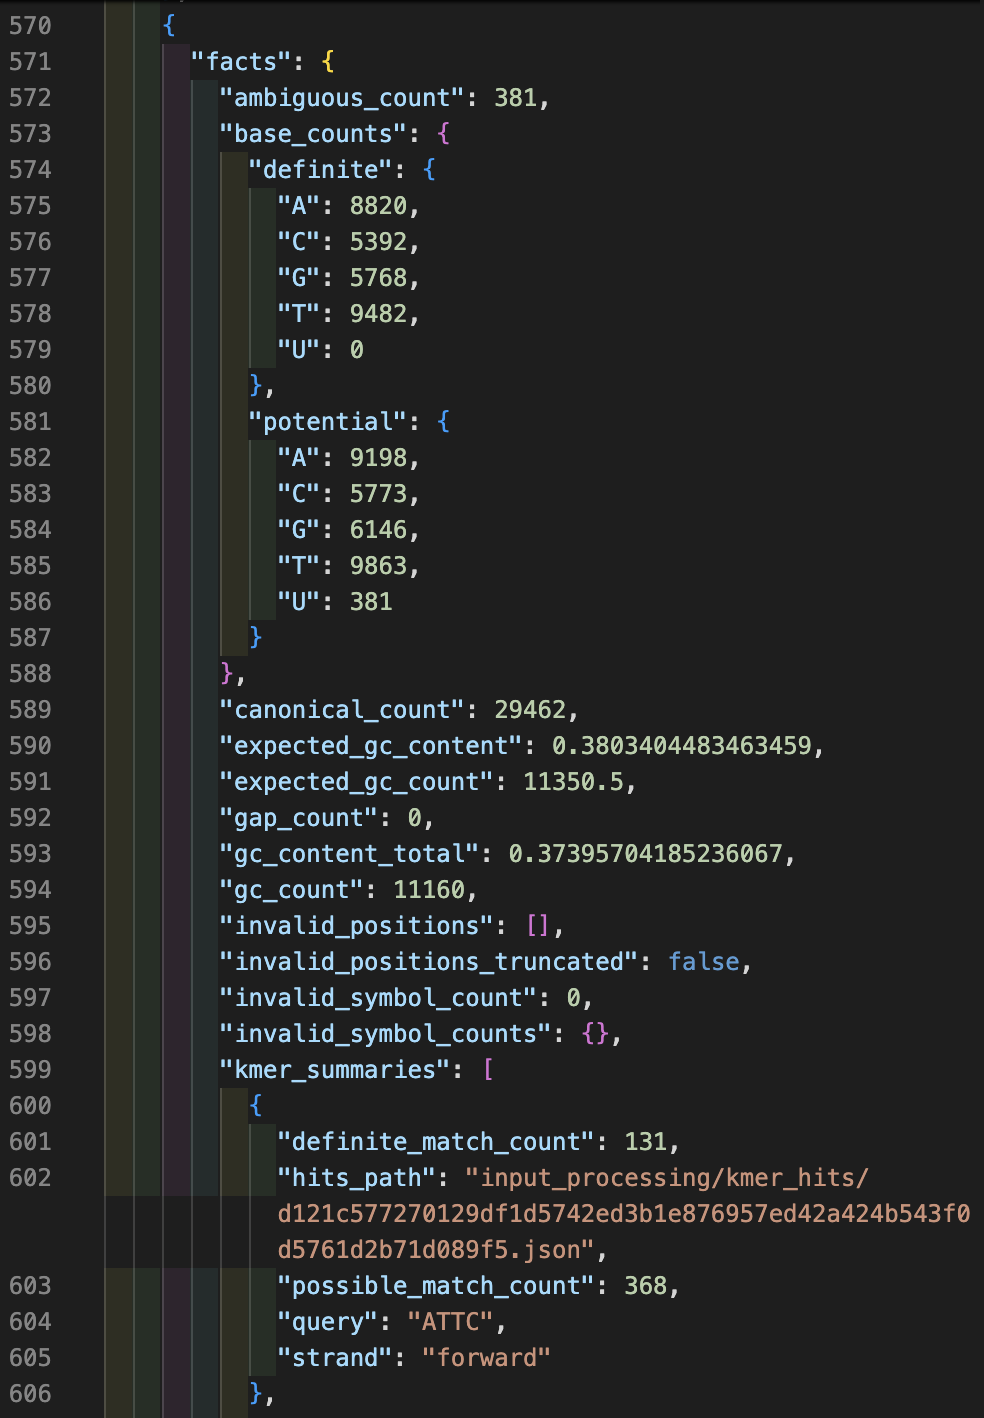
\includegraphics[width=\textwidth]{input-processing-statistics.png}
        \caption{Фрагмент статистичких карактеристика секвенце}
        \label{fig:input-processing-statistics}
    \end{subfigure}
    \hfill
    \begin{subfigure}[t]{0.49\textwidth}
        \centering
        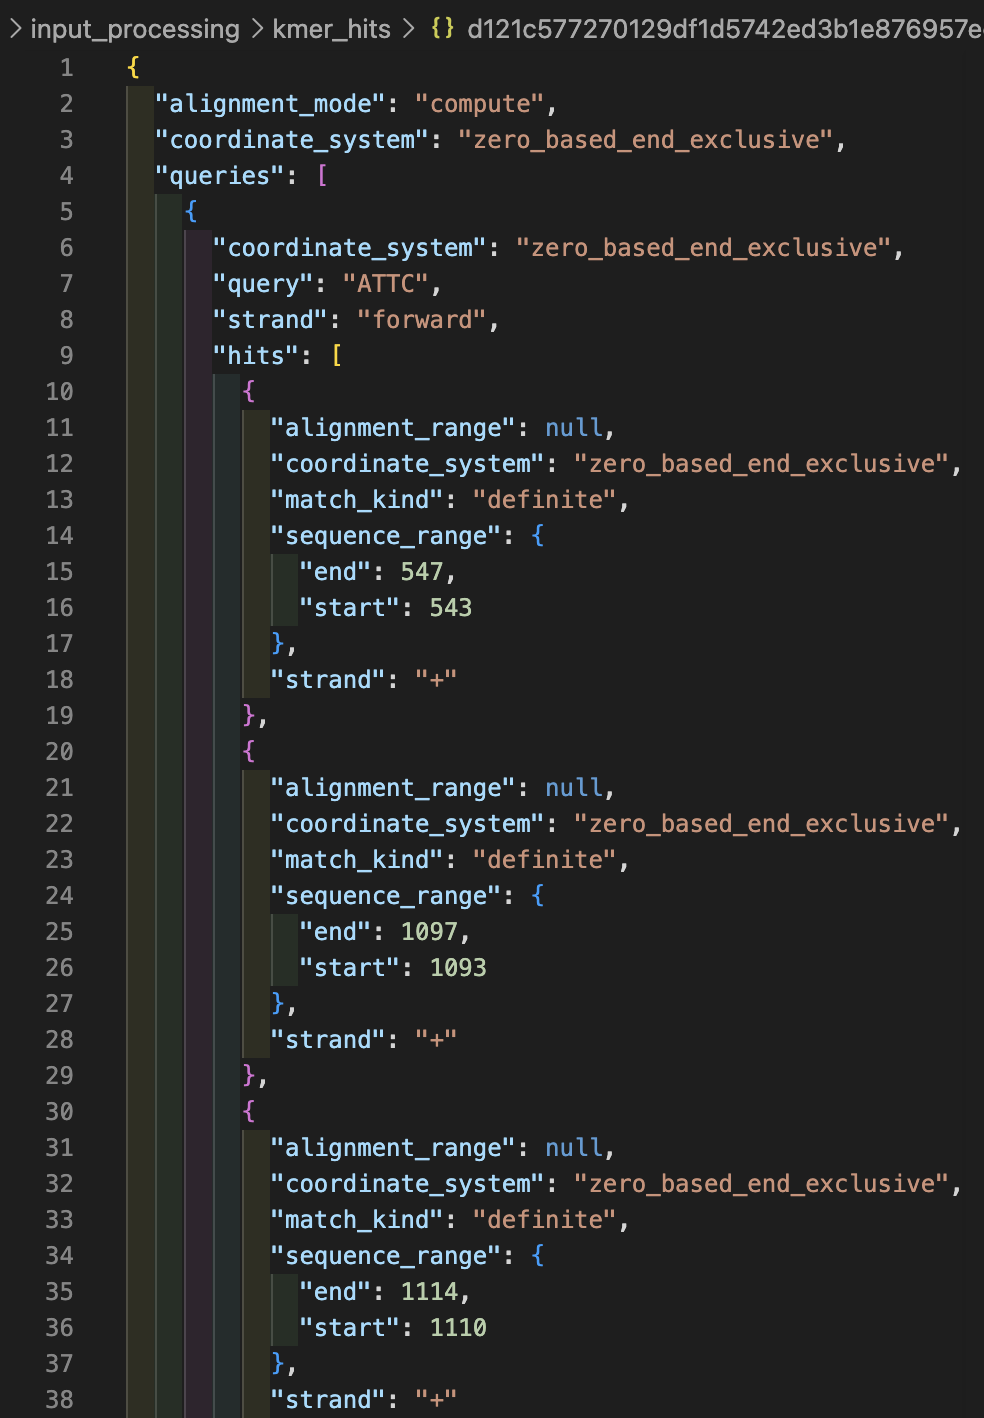
\includegraphics[width=\textwidth]{input-processing-kmer-results.png}
        \caption{Фрагмент резултата претраге \(k\)-мера}
        \label{fig:input-processing-kmers}
    \end{subfigure}

    \caption{Пример резултата фазе \texttt{input\_processing}}
    \label{fig:input-processing-results}
\end{figure}

Начин обраде поравнања одређен је конфигурацијом аналитичког задатка. У режиму \textit{compute} систем формира вишеструко поравнање коришћењем алата \textit{MAFFT}, при чему се задата референтна секвенца користи као основа за референтно поравнање и у наредним фазама које захтевају референтни координатни систем. У режиму \textit{prealigned} користе се већ поравнате улазне секвенце, чија се компатибилност претходно проверава; уколико је референтна секвенца задата, она се и у овом режиму користи у фазама које захтевају референтни координатни систем. У режиму \textit{none} фаза поравнања се не извршава, па се изостављају и наредне аналитичке фазе којима су поравнате секвенце неопходне као улаз.

Над формираним поравнањем извршава се фаза \texttt{comparative\_analysis}, која обухвата израчунавање статистичких показатеља и упоредну анализу изабраних парова секвенци. Поређења се могу извршавати за цео скуп, унутар група секвенци дефинисаних од стране корисника или за експлицитно задате парове. Добијени резултати користе се за визуелизацију и формирање извештаја.

Фаза \texttt{distance\_matrix} из поравнатих секвенци формира квадратну матрицу генетичких растојања. Добијене вредности представљају основу за процену међусобне сличности узорака и за каснију реконструкцију њихових еволуционих односа. Матрица се чува у машински читљивим форматима, што омогућава њен непосредан приказ, извоз или даљу обраду без поновног израчунавања претходних фаза.

На основу матрице растојања фаза \texttt{phylogenetic\_tree} формира филогенетско стабло применом методе \textit{Neighbor Joining}. Резултат се чува у стандардном формату \textit{Newick}\footnote{\textit{\textbf{Newick}} је текстуални формат за представљање структуре филогенетског стабла помоћу угњеждених заграда, назива чворова и, по потреби, дужина грана.}, као и у структуираном облику погодном за визуелизацију у графичким интерфејсима. Имплементација обезбеђује детерминистичко извршавање аналитичког задатка, тако да се при истим улазним подацима и конфигурацији добија исти резултат.

Након формирања матрице растојања могуће је извршити и фазу \texttt{clade\_detection}, у којој се узорци групишу према задатом максималном растојању унутар групе. При томе се користе вредности из матрице парних генетичких растојања, у којој се растојање између две секвенце рачуна као однос броја позиција на којима се поравнате секвенце разликују и укупног броја позиција које се у том поређењу узимају у обзир.


\subsection{Чување стања, међурезултата и резултата аналитичког задатка}
Чување података у систему \textit{JELICA} реализовано је применом хибридног модела. Метаподаци о аналитичким задацима чувају се у бази података \textit{SQLite}, док се конфигурације, улазни подаци и резултати њиховог извршавања смештају у систем датотека. За сваки задатак формира се засебан радни директоријум који садржи његову нормализовану конфигурацију, податке и резултате појединачних аналитичких фаза. Пример фрагмента нормализоване конфигурације аналитичког задатка приказан је на слици~\ref{fig:normalized-task-configuration}.

Резултати завршених фаза објављују се тек након успешног формирања свих обавезних међурезултата и манифеста. На тај начин међурезултати остају раздвојени од завршних и систем може да настави прекинути аналитички задатак од последње успешно завршене фазе.

Завршни резултати аналитичког задатка обједињују се у датотеку формата \texttt{.јelica}, интерно реализовану као компримована архивска структура. У наставку се ова датотека означава као \textbf{пакет са резултатима аналитичког задатка}, јер поред самих резултата садржи и пратеће податке неопходне за њихово поновно учитавање и приказ. Пакет садржи нормализоване улазне секвенце, нормализовану конфигурацију задатка, резултате аналитичких фаза, њихове манифесте, дијагностичке податке и контролне суме за проверу интегритета. Као једини кориснички изменљив додатак дозвољена је датотека \texttt{./NOTES.txt}. Пример структуре садржаја формираног пакета приказан је на слици~\ref{fig:jelica-package-structure}.

\begin{figure}[htbp]
    \centering

    \begin{subfigure}[t]{0.54\textwidth}
        \centering
        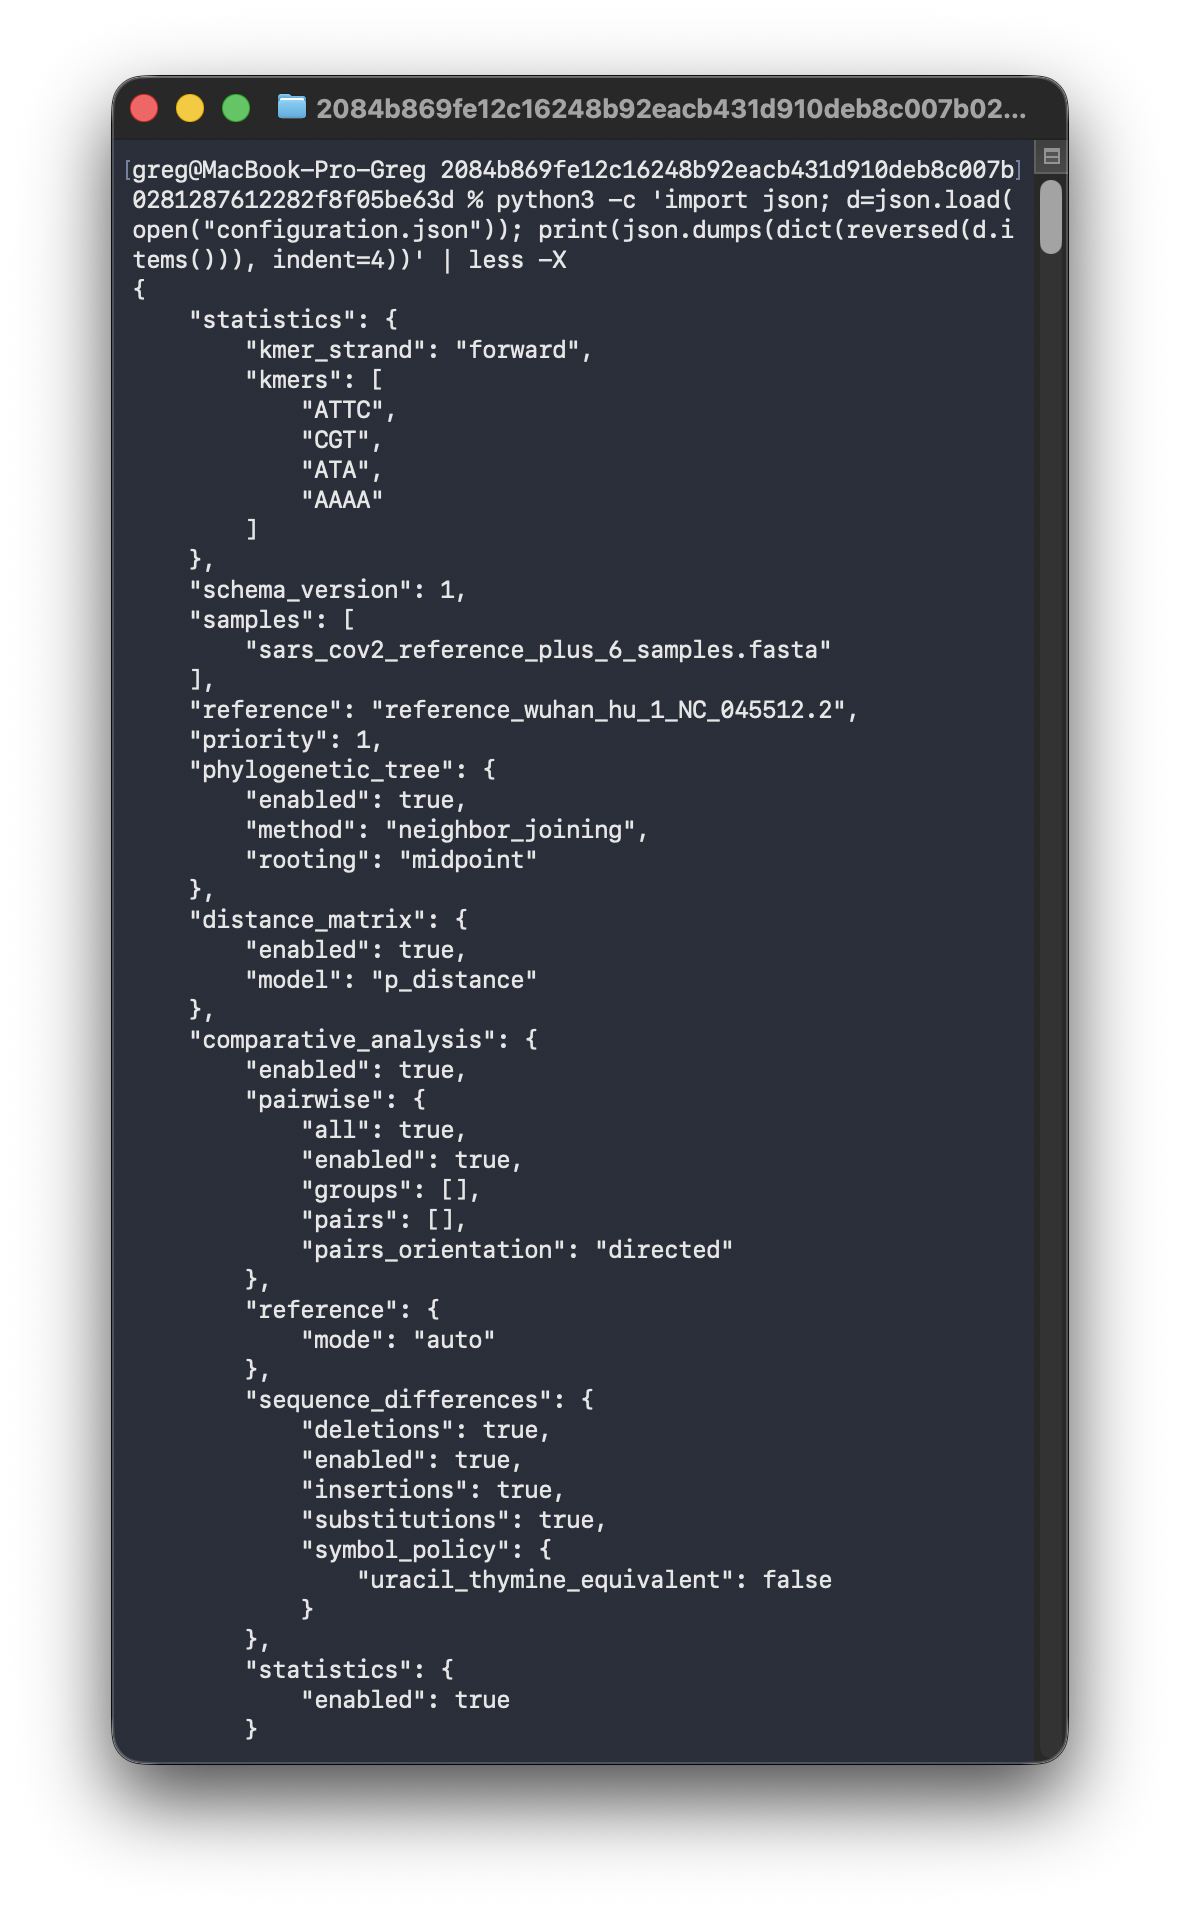
\includegraphics[width=\textwidth]{normalized-task-configuration.png}
        \caption{Фрагмент нормализоване конфигурације аналитичког задатка}
        \label{fig:normalized-task-configuration}
    \end{subfigure}
    \hfill
    \begin{subfigure}[t]{0.45\textwidth}
        \centering
        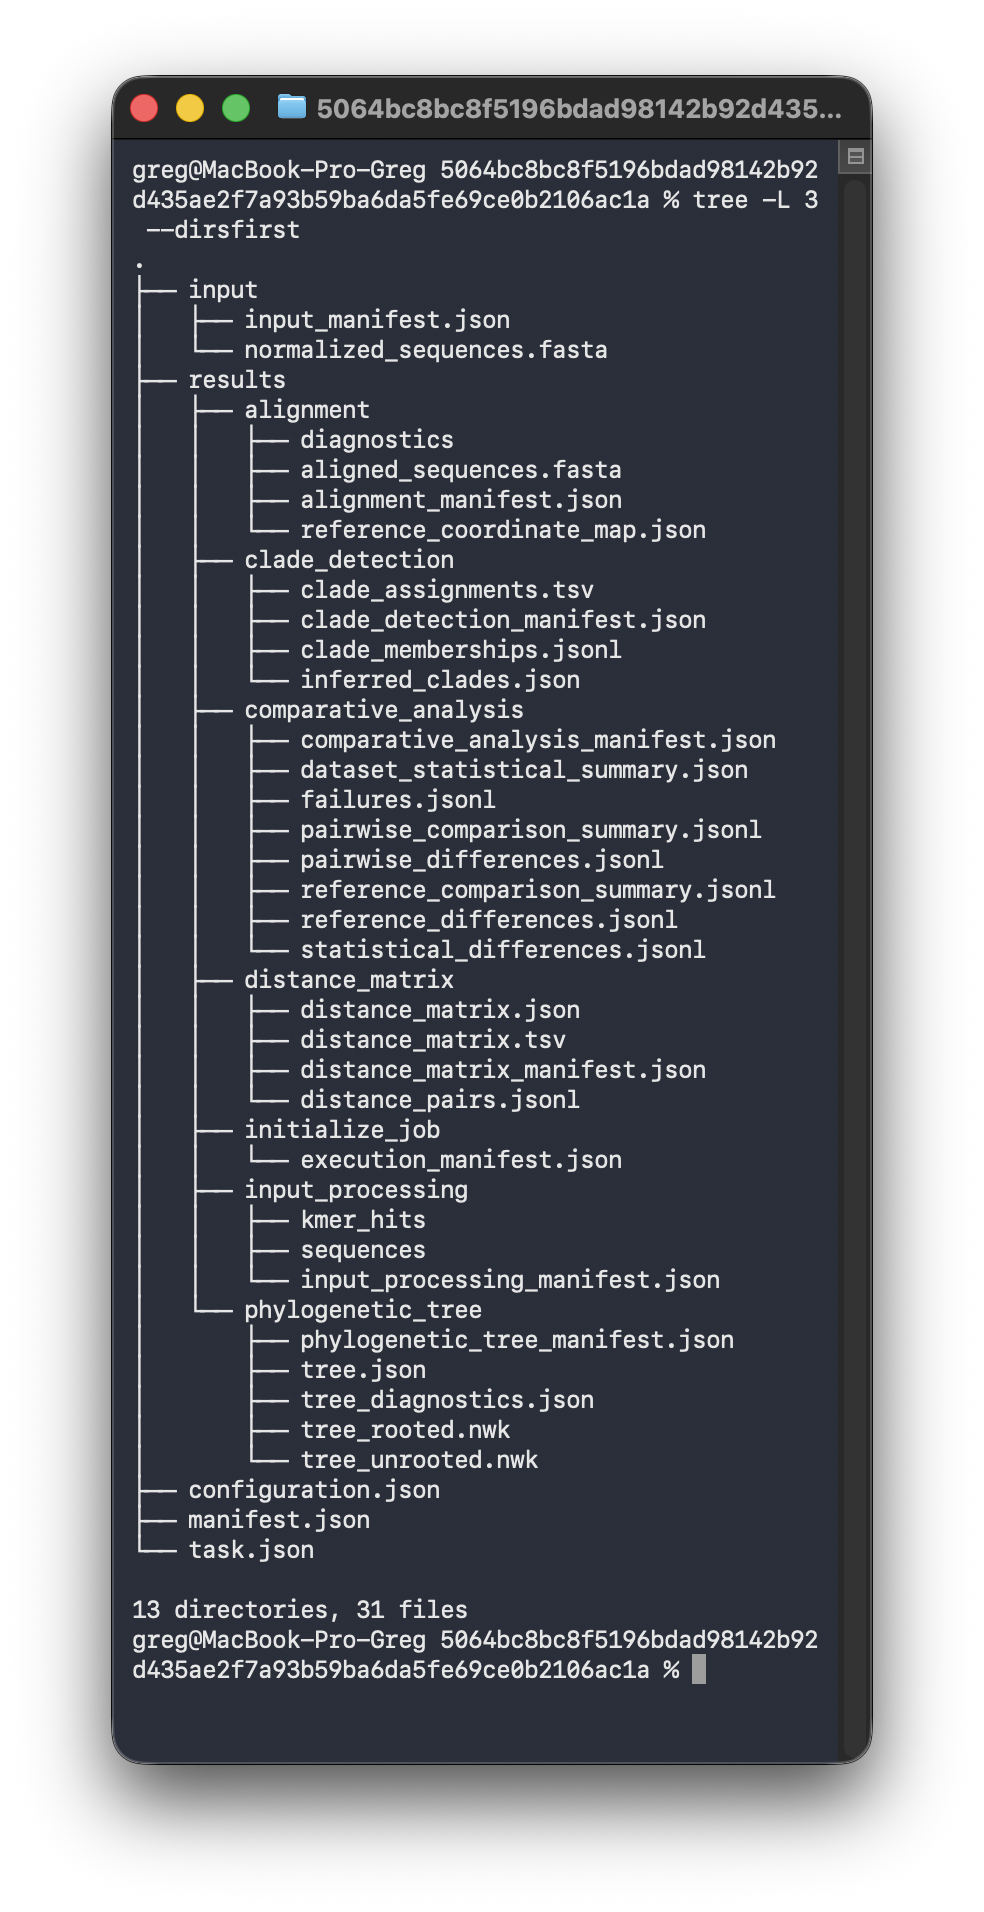
\includegraphics[width=\textwidth]{jelica-package-structure.png}
        \caption{Структура садржаја пакета резултата формата \texttt{.jelica}}
        \label{fig:jelica-package-structure}
    \end{subfigure}

    \caption{Чување конфигурације аналитичког задатка и структура пакета резултата}
    \label{fig:task-configuration-and-result-package}
\end{figure}

Формирани и увезени пакети са резултатима аналитичког задатка организују се у директоријуму \texttt{result\_packages}.

На основу структурираног садржаја пакета формирају се \textit{HTML} и \textit{PDF} извештаји, интерактивне визуелизације и други формати датотека за извоз резултата, без измене садржаја самог пакета. Исти пакет се зато може користити у интерфејсу командне линије, веб-платформи и десктоп апликацији.


\subsection{Поузданост, опоравак и праћење тока извршавања}
Захтеви за поузданост, опоравак и праћење тока извршавања дефинисани у потпоглављу~\ref{sec:specification-of-system-quality-criteria} имплементирани су кроз проверу конфигурације и улазних података, контролу дозвољених прелаза између стања аналитичких задатака и трансакционо ажурирање регистра. Проверавају се и резултати појединачних аналитичких фаза, тако да наредна фаза не користи непотпуне или неисправно формиране податке.

При неуспешном креирању задатка привремени подаци се уклањају, док при прекиду започетог аналитичког задатка резултати успешно завршених фаза остају сачувани и могу се користити при настављању. Грешке су изоловане у оквиру појединачног задатка и не прекидају извршавање других задатака.

Грешке, упозорења и други значајни догађаји бележе се у структуираном облику са временом настанка, нивоом критичности, бројчаним кодом, извором и контекстом. За различите компоненте система резервисани су засебни опсези кодова, приказани у табели~\ref{tab:event-code-ranges}, док се догађаји аналитичког задатка повезују са његовим идентификатором. Интерни изузеци претварају се у структуриране грешке погодне за приказ у корисничким интерфејсима, без откривања интерних техничких детаља. Структурирани дневници омогућавају реконструкцију тока извршавања и утврђивање фазе у којој је проблем настао.

\begin{table}[htbp]
    \centering
    \caption{Опсези кодова догађаја у систему \textit{JELICA}}
    \label{tab:event-code-ranges}
    \begin{tabular}{|l|c|}
        \hline
        \textbf{Компонента} & \textbf{Опсег кодова} \\
        \hline
        Резервисано за будуће системске догађаје (\texttt{SYSTEM\_*}) & 1000--1999 \\
        \hline
        Аналитичко језгро (\texttt{CORE\_*}) & 2000--2999 \\
        \hline
        Интерфејс командне линије (\texttt{CLI\_*}) & 3000--3999 \\
        \hline
        Серверска компонента веб-платформе (\texttt{SERVER\_*}) & 4000--4999 \\
        \hline
        Веб-платформа (\texttt{WEB\_*}) & 5000--5999 \\
        \hline
        Десктоп апликација (\texttt{DESKTOP\_*}) & 6000--6999 \\
        \hline
        Резервисано & 7000--9999 \\
        \hline
    \end{tabular}
\end{table}


\subsection{Кориснички интерфејси}
Систем \textit{JELICA} доступан је преко \textbf{интерфејса командне линије}, \textbf{веб-платформе} и \textbf{десктоп апликације}. Основни облици њиховог коришћења и однос према заједничком аналитичком језгру описани су у потпоглављу~\ref{sec:forms-of-using-the-system}. Веб-платформа и десктоп апликација подржавају локализацију корисничког интерфејса на енглески, руски и српски језик, при чему је српски доступан на ћириличком и латиничком писму. Интерфејс командне линије користи енглески језик, док се извештаји могу генерисати на сва четири подржана језичка и писмена облика.

При реализацији корисничких интерфејса посебна пажња посвећена је приступачности. Веб-платформа развијена је са циљним нивоом усаглашености \textit{AA} према смерницама \textit{Web Content Accessibility Guidelines 2.2} (\textit{WCAG 2.2})\footnote{\textit{\textbf{Web Content Accessibility Guidelines}} (\textit{WCAG}) представља међународни стандард приступачности веб-садржаја који развија \textit{World Wide Web Consortium} (\textit{W3C}) у оквиру иницијативе \textit{Web Accessibility Initiative} (\textit{WAI}). Стандард дефинише смернице и проверљиве критеријуме намењене побољшању приступачности веб-страница и веб-апликација особама са визуелним, слушним, моторичким, говорним, когнитивним и другим облицима инвалидитета. Смернице су организоване око четири основна принципа: садржај треба да буде опажљив, употребљив, разумљив и робустан. Критеријуми усаглашености подељени су на нивое \textit{A}, \textit{AA} и \textit{AAA}; усаглашеност са нивоом \textit{AA} подразумева испуњавање свих критеријума нивоа \textit{A} и \textit{AA}. Верзија \textit{WCAG 2.2} објављена је као препорука \textit{W3C}-а 5. октобра 2023. године и представља актуелну верзију стандарда \textit{WCAG 2} у време израде овог рада.~\cite{wcag22}}, док се применљиви принципи истог стандарда користе и приликом пројектовања десктоп апликације. То обухвата, између осталог, рад помоћу тастатуре, видљив фокус активног елемента, довољан контраст, семантички структуриран садржај и избегавање ослањања искључиво на боју за преношење значења.

Приступачност интерфејса командне линије примењује се у складу са ограничењима терминалног окружења. Боје и декоративни симболи нису неопходни за разумевање резултата и могу се искључити, док су значајне поруке увек доступне и у текстуалном облику. Графички интерфејси прилагођавају распоред различитим величинама екрана и не захтевају употребу показивачког уређаја за основне операције.

Приликом избора технологија и реализације интерфејса тежи се и компатибилности са различитим рачунарима, оперативним системима и веб-прегледачима. Интерфејси не претпостављају употребу високоперформансног корисничког уређаја, а зависност од функција доступних искључиво у најновијим верзијама платформи избегава се када за то не постоји функционална потреба. На тај начин се подржава широк спектар актуелних и старијих система, у мери у којој то не нарушава исправност рада апликације.


\subsubsection{Интерфејс командне линије}
Интерфејс командне линије реализован је као засебна апликација \texttt{jelica-cli}, која након инсталације омогућава коришћење команде \texttt{jelica} из било ког директоријума на рачунару на којем је инсталирана локална верзија система. Он представља непосредну приступну тачку локалној верзији аналитичког језгра и не садржи сопствену аналитичку логику. Његов задатак је да корисничке команде и параметре претвори у структуриране захтеве језгра и да добијене резултате прикаже у облику погодном за интерактивну или машинску употребу. Интерфејс командне линије омогућава подешавање локалног окружења, креирање, покретање, праћење, паузирање, настављање и отказивање аналитичких задатака, њихово клонирање и приступ сачуваним пакетима резултата.

Већина појединачних команди интерфејса командне линије извршава засебне операције над аналитичким задацима, што је погодно за машинску интеракцију и аутоматизацију. За најчешћи интерактивни сценарио употребе уведена је команда \texttt{jelica analyze}, која у једном позиву обједињује креирање задатка (\texttt{jelica tasks create}), његово покретање (\texttt{jelica tasks start}) и праћење извршавања (\texttt{jelica tasks watch}). Улазни извори задају се позиционим аргументима, док се конфигурација може проследити у \textit{JSON} датотеци, параметрима командне линије или комбинацијом оба начина. За угнежђене параметре користи се тачкаста нотација, при чему вредности задате командом имају приоритет над вредностима из конфигурационе датотеке. Структура команде \texttt{jelica analyze} и начини задавања њених параметара приказани су на слици~\ref{fig:analyze-command-structure-schematic}, док је пример њеног покретања и извршавања аналитичког задатка приказан на слици~\ref{fig:jelica-analyze-results}.

\begin{figure}[htbp]
    \centering

    \begin{subfigure}{0.95\textwidth}
        \centering
        
\includegraphics[width=\textwidth]{analyze-command-structure-schematic.png}
        \caption{Шематски приказ структуре команде \texttt{jelica analyze}}
        \label{fig:analyze-command-structure-schematic}
    \end{subfigure}

    \vspace{0.5cm}

    \begin{subfigure}{0.9\textwidth}
        \centering
        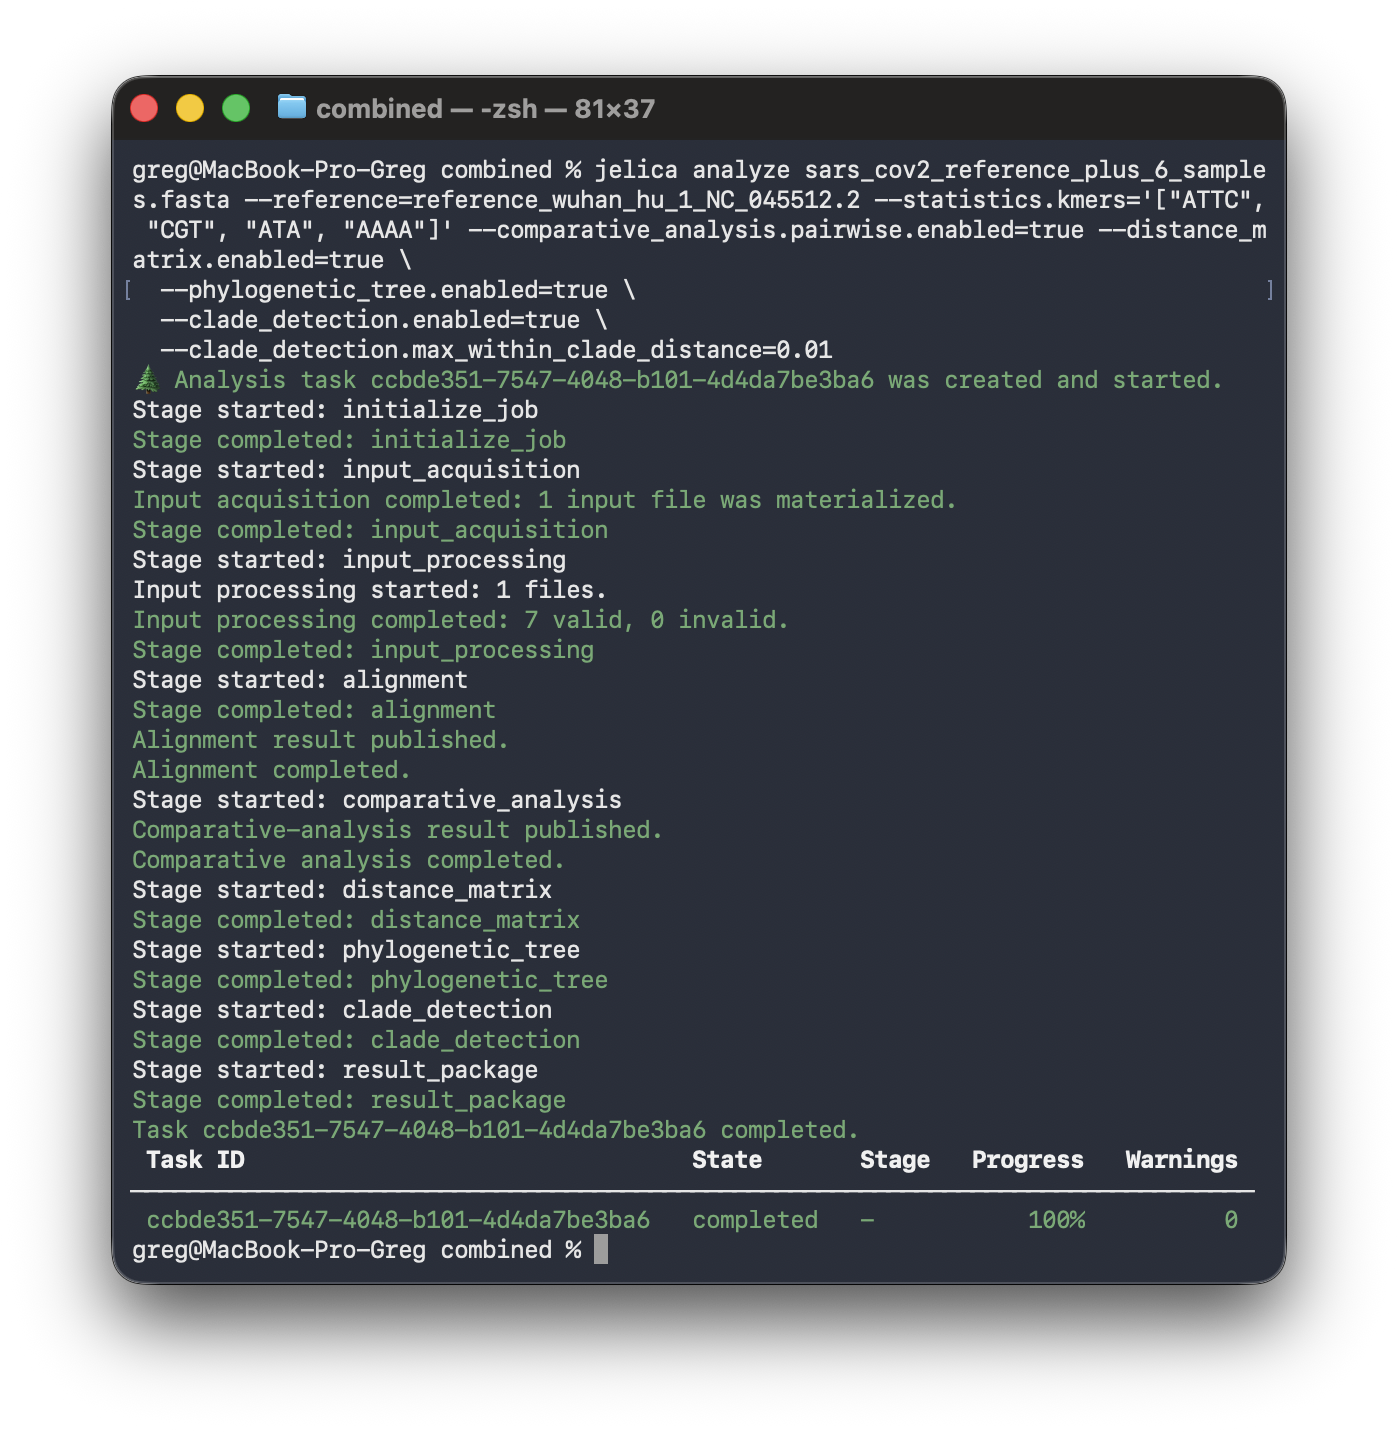
\includegraphics[width=\textwidth]{jelica-analyze-results.png}
        \caption{Пример покретања и извршавања аналитичког задатка командом \texttt{jelica analyze}}
        \label{fig:jelica-analyze-results}
    \end{subfigure}

    \caption{Структура и пример употребе команде \texttt{jelica analyze}}
    \label{fig:jelica-analyze}
\end{figure}

Током извршавања \textit{CLI} приказује идентификатор задатка, тренутно стање, активну фазу и напредак, као и значајне информационе и дијагностичке поруке. Недозвољени параметри, грешке у конфигурацији и недопуштени прелази између стања приказују се без откривања интерних техничких детаља извршавања.

За аутоматизовану употребу команде подржавају машински читљив излаз и једнозначне излазне кодове. Захваљујући томе \textit{JELICA} се може укључити у скрипте, програмске омотаче и друге аутоматизоване процесе без анализирања текста намењеног човеку. Исти скуп основних команди доступан је у оперативним системима \textit{macOS}, \textit{Windows} и \textit{Linux}.


\subsubsection{Веб-платформа}
Веб-платформа пружа графички приступ функцијама система без потребе за локалним радом у терминалу. Кориснички интерфејс омогућава организовање аналитичких задатака у оквиру пројеката, додавање улазних података и управљање њима, подешавање параметара аналитичког задатка, праћење његовог извршавања и интерактиван преглед добијених резултата.

Пројекат представља организациони ниво специфичан за веб-платформу и не мења модел аналитичког задатка у језгру. Један пројекат може да обједини повезане улазне податке, више аналитичких задатака и њихове резултате, али и да омогући заједнички рад више корисника над истим анализама. Корисници са одговарајућим правима могу у оквиру пројекта креирати и мењати задатке, покретати, паузирати и настављати њихово извршавање, као и остављати коментаре другим учесницима. На тај начин пројекти истовремено служе за организацију истраживачких података и основну сарадњу корисника у оквиру веб-платформе.

При покретању аналитичког задатка веб-интерфејс формира конфигурацију аналитичког задатка у истом формату као и остали интерфејси система и прослеђује је серверској компоненти. Архитектонски начин комуникације веб-платформе са аналитичким језгром описан је у потпоглављу~\ref{sec:general-system-architecture}. Кориснику се током извршавања приказују тренутно стање аналитичког задатка и напредак његовог извршавања. Корисник може прилагодити обавештења о значајним догађајима у систему и начин њиховог достављања — у самом интерфејсу, путем електронске поште или преко месинџера \textit{WhatsApp} и \textit{Telegram}. Иако је подршка за \textit{Viber} била предвиђена функционалном спецификацијом система у потпоглављу~\ref{sec:functional-specification}, током имплементације се од њене реализације одустало због комерцијалних услова коришћења програмског интерфејса овог сервиса и фиксних трошкова одржавања бота.

Резултати се у веб-интерфејсу приказују комбинацијом табеларних података, сажетака и интерактивних визуелизација. На основу пакета резултата могуће је формирати и преузети извештаје и извозне датотеке, као и преузети саму датотеку \texttt{.jelica} ради локалног чувања или отварања у десктоп апликацији.

Поред аналитичких функција, веб-платформа служи и као централно место за преузимање локалних верзија система са \textit{CLI} и десктоп интерфејсом, приступ документацији и информацијама о пројекту, као и за подршку и слање повратних информација.


\subsubsection{Десктоп апликација}
Десктоп апликација обезбеђује графички рад са локалном верзијом система и кориснику поједностављује креирање аналитичких задатака, подешавање њихових параметара и управљање редом извршавања. Она користи исти визуелни систем и основне компоненте интерфејса као веб-платформа, чиме се обезбеђује уједначен начин навигације и рада са резултатима. Комуникација са аналитичким језгром остварује се преко машинског интерфејса \textit{CLI}-ја, који служи као посреднички слој између десктоп апликације и модула \textit{Core}.

Апликација омогућава и приказ структурираних резултата, филогенетских стабала, статистичких података и извештаја. Формат \texttt{.jelica} може бити повезан са десктоп апликацијом, тако да се пакет резултата отвара непосредно као документ система \textit{JELICA}, без ручног приступа његовој унутрашњој структури.


\subsection{Инфраструктура веб-платформе}
За разлику од локалних варијанти система, веб-платформа обухвата додатни инфраструктурни слој за мрежни приступ, истовремени рад више корисника и трајно чување њихових података. Јавно доступна верзија система користи протокол \textit{HTTPS}, док су кориснички интерфејс, серверски слој и аналитичко извршавање логички раздвојени.

Комуникација серверског слоја са аналитичким језгром организована је у складу са архитектуром описаном у потпоглављу~\ref{sec:general-system-architecture}. Аналитички задатак се извршава независно од животног циклуса појединачног \textit{HTTP} захтева, док се ажурирања стања и напретка активних задатака веб-клијенту прослеђују преко \textit{WebSocket} везе.

Аналитички задаци и пакети резултата повезују се са одговарајућим пројектима и корисничким налозима, док серверска апликација контролише приступ подацима и ограничења расположивог простора за њихово чување. Раздвајање веб-инфраструктуре од аналитичког језгра омогућава независну инсталацију и скалирање веб-платформе без измене аналитичких алгоритама и формата резултата.


\subsection{Корисничка документација}
Корисничка документација обухвата опис техничке организације система и практично упутство за његово коришћење. Доступна је у оквиру веб-платформе и десктоп апликације, са могућностима брзе навигације и претраге, и локализована је на исте језичке и писмене варијанте као графички кориснички интерфејси. При њеној реализацији примењују се исти принципи приступачности као и у осталим деловима корисничког интерфејса.

Све варијанте документације формирају се из заједничког извора садржаја, чиме се избегава паралелно одржавање више независних верзија. За локални рад преко интерфејса командне линије аутоматски се формира \textit{PDF} верзија истог садржаја, која се испоручује уз локалну инсталацију и доступна је за преузимање са веб-платформе.


\chapter{Закључак}
У оквиру овог рада развијен је софтверски систем \textit{JELICA}, који обједињује различите кораке упоредне анализе геномских секвенци у јединствен аналитички ток. Аутоматизација припреме улазних података, поравнања, поређења и филогенетске анализе смањује потребу за ручним преношењем података између независних алата и обезбеђује доследан начин извршавања и чувања резултата. Преносиви формат \texttt{.jelica} омогућава чување, размену и накнадну употребу целокупног резултата спроведене анализе.

Систем је доступан преко интерфејса командне линије, веб-платформе и десктоп апликације, чиме је прилагођен и аутоматизованој и интерактивној употреби. Веб-верзија омогућава рад без локалне инсталације, док локалне варијанте омогућавају обраду података на сопственом рачунару. Изворни код је јавно доступан и, у складу са лиценцом, може се користити, мењати, проширивати и укључивати у друге системе уз очување података о оригиналном пројекту и ауторству, док су ограничени препродаја самог система и комерцијална употреба заснована превасходно на њему.

Даљи развој може обухватити подршку за додатне методе и алате за поравнање секвенци, развој сопственог алгоритма поравнања и замену рачунарски захтевних операција заснованих на библиотеци \textit{Biopython} ефикаснијим сопственим имплементацијама. Планирано је и проширење метода за израчунавање генетичких растојања и филогенетску анализу, унапређење паралелног и дистрибуираног извршавања, додавање нових локализација и програмски приступ јавној веб-верзији путем јавног \textit{API}-ја.
% ------------------------------------------------------------------------------

% ------------------------------------------------------------------------------
% Literatura
% ------------------------------------------------------------------------------
\literatura

% ==============================================================================
% Završni deo teze i prilozi
\backmatter
% ==============================================================================

% ------------------------------------------------------------------------------
% Biografija kandidata
\begin{biografija}
Григории Рогов рођен је 12. августа 1998. године у Москви, у Русији. Средњу школу са појачаном наставом из биологије и хемије завршио је у Москви 2016. године. Самостално је стекао знања из програмирања, пре свега у програмском језику \textit{JavaScript}, а професионалну каријеру започео је 2018. године у компанији \textit{STREAM LABS}, која се бави развојем хардверских и софтверских решења за телевизијску и радијску опрему, као и системе видео-надзора. Исте године уписао је Московски технички универзитет веза и информатике, на студијски програм „Информациони системи и технологије“, који је завршио 2023. године са одличним успехом. Тема дипломског рада била је „Развијање модела гранања за систем контроле верзија Git“.

Године 2022. преселио се са супругом у Београд, где је наставио професионални рад као самостални предузетник, пружајући услуге развоја софтвера. Током професионалног рада бавио се пре свега развојем веб-апликација и корисничких интерфејса. Мастер академске студије на студијском програму Информатика Математичког факултета Универзитета у Београду уписао је 2024. године.
\end{biografija}
% ------------------------------------------------------------------------------

\end{document} 